\documentclass[12pt,a4paper,oneside]{report}

% ---------------------------------------------------------------------------
% Thesis data
% ---------------------------------------------------------------------------
\newcommand{\ThesisTitle}{Training-Free Adaptive Control of Detector and Tracker Operating Points for Multi-Object Tracking}
\newcommand{\ThesisAuthor}{Ahmed Gouda Ismail}
\newcommand{\ThesisDegree}{Master of Science}
\newcommand{\ThesisField}{Computer Engineering}
\newcommand{\ThesisDepartment}{Computer Engineering and Artificial Intelligence Department}
\newcommand{\ThesisInstitution}{Military Technical College}
\newcommand{\ThesisCity}{Cairo, Egypt}
\newcommand{\ThesisYear}{2026}
\newcommand{\SupervisorOne}{Mohamed S. Mohamed}
\newcommand{\SupervisorOneAffil}{Computer Engineering and Artificial Intelligence Department, Military Technical College}
\newcommand{\SupervisorTwo}{Tarek Ahmed Mahmoud}
\newcommand{\SupervisorTwoAffil}{Computer Engineering Department, Egypt University of Informatics}
\newcommand{\PaperOneStatus}{submitted}
\newcommand{\PaperTwoStatus}{submitted}
% ---------------------------------------------------------------------------
% Packages
% ---------------------------------------------------------------------------
\usepackage[T1]{fontenc}
\usepackage{lmodern}
\usepackage[english]{babel}
\usepackage{amsmath,amssymb}
\usepackage[a4paper,left=3.0cm,right=2.5cm,top=2.5cm,bottom=2.5cm,headheight=15pt]{geometry}
\usepackage{setspace}
\onehalfspacing
\usepackage{graphicx}
\usepackage{booktabs}
\usepackage{adjustbox}
\usepackage{rotating}
\usepackage{longtable}
\usepackage{array}
\usepackage{enumitem}
\setlist{itemsep=2pt,topsep=4pt}
\usepackage[labelfont=bf,font=small]{caption}
\usepackage{algorithm}
\usepackage{algpseudocode}
\usepackage{pdfpages}
\usepackage{tikz}
\usetikzlibrary{positioning,arrows.meta,fit,backgrounds,calc}
\usepackage[numbers,sort&compress]{natbib}
\usepackage{fancyhdr}
\usepackage[nottoc]{tocbibind}
\usepackage{emptypage}
\usepackage[hidelinks,unicode]{hyperref}
\hypersetup{pdftitle={\ThesisTitle},pdfauthor={\ThesisAuthor}}
\setlength{\emergencystretch}{3em}
\setcounter{tocdepth}{2}
\setcounter{secnumdepth}{3}

\pagestyle{fancy}
\fancyhf{}
\renewcommand{\headrulewidth}{0.4pt}
\fancyhead[R]{\small\nouppercase{\leftmark}}
\fancyfoot[C]{\thepage}
\fancypagestyle{plain}{\fancyhf{}\renewcommand{\headrulewidth}{0pt}\fancyfoot[C]{\thepage}}

% Tables and figures are numbered within chapters.
\numberwithin{equation}{chapter}

\begin{document}

\pagenumbering{roman}
\pagestyle{plain}
\begin{titlepage}
\centering
\thispagestyle{empty}
{\large\ThesisInstitution\par}
{\normalsize\ThesisDepartment\par}
\vspace{2.2cm}
{\LARGE\bfseries\setstretch{1.3}\ThesisTitle\par}
\vspace{1.8cm}
{\normalsize By\par}
\vspace{0.3cm}
{\Large\ThesisAuthor\par}
\vspace{1.8cm}
{\normalsize A thesis submitted in partial fulfillment of the requirements\\ for the degree of\par}
\vspace{0.3cm}
{\large\ThesisDegree\ in \ThesisField\par}
\vspace{1.8cm}
{\normalsize Supervised by\par}
\vspace{0.4cm}
{\large\SupervisorOne\par}
{\small\SupervisorOneAffil\par}
\vspace{0.4cm}
{\large\SupervisorTwo\par}
{\small\SupervisorTwoAffil\par}
\vfill
{\normalsize\ThesisCity\par}
{\normalsize\ThesisYear\par}
\end{titlepage}

\chapter*{Approval Sheet}
\thispagestyle{plain}
\begin{center}
{\large\bfseries\ThesisTitle\par}
\vspace{0.4cm}
By\par
{\large\ThesisAuthor\par}
\vspace{0.3cm}
A thesis submitted in partial fulfillment of the requirements for the degree of \ThesisDegree\ in \ThesisField
\end{center}

\vspace{0.3cm}
\noindent\textbf{Examination Committee}

\vspace{0.4cm}
\renewcommand{\arraystretch}{2.0}
\noindent\begin{tabular}{@{}p{0.5\textwidth}p{0.4\textwidth}@{}}
Name & Signature \\
\hline
\rule{0pt}{1.2em} & \\
\hline
\rule{0pt}{1.2em} & \\
\hline
\rule{0pt}{1.2em} & \\
\hline
\rule{0pt}{1.2em} & \\
\hline
\end{tabular}

\vspace{0.5cm}
\noindent\textbf{Supervisors}

\vspace{0.4cm}
\noindent\begin{tabular}{@{}p{0.5\textwidth}p{0.4\textwidth}@{}}
Name & Signature \\
\hline
\SupervisorOne & \\
\hline
\SupervisorTwo & \\
\hline
\end{tabular}
\renewcommand{\arraystretch}{1.0}

\vspace{0.5cm}
\noindent Date: \rule{5cm}{0.4pt}

\chapter*{Declaration}
\thispagestyle{plain}
I declare that this thesis is my own work and that it has not been submitted for any other degree or qualification at this or any other institution. The work was carried out in the \ThesisDepartment, \ThesisInstitution, under the supervision of \SupervisorOne\ and \SupervisorTwo. Where the work of others is used, it is acknowledged by citation. Parts of Chapter~\ref{ch:background} were published in a conference paper, and Chapters~\ref{ch:scene} and~\ref{ch:layer} are based on two journal manuscripts written with my supervisors; these publications are listed on page~\pageref{sec:publications}.

\vspace{1.5cm}
\noindent\begin{tabular}{@{}l@{}}
\rule{6cm}{0.4pt}\\
\ThesisAuthor\\
\ThesisYear
\end{tabular}

\chapter*{Acknowledgments}
\thispagestyle{plain}
I am grateful to my supervisors, \SupervisorOne\ and \SupervisorTwo, for their guidance, their careful reading of every result, and their insistence on evaluating the work honestly. I thank the \ThesisDepartment\ of the \ThesisInstitution\ for its support throughout this research.

I also thank the authors of the published trackers and detectors evaluated in this thesis for releasing their code, weights, and detections, and the maintainers of the VisDrone, UAVDT, MOT17, KITTI, and DanceTrack benchmarks and of the TrackEval library, without whom a reproducible evaluation would not have been possible.

Finally, I thank my family for their patience and encouragement.

\chapter*{Abstract}
\thispagestyle{plain}
\addcontentsline{toc}{chapter}{Abstract}

Multi-object tracking by detection is the standard way to obtain persistent object identities in video: a detector proposes scored boxes in every frame, and an online tracker associates them over time. Both components are governed by a small number of operating-point parameters, namely the detector's confidence threshold, suppression threshold, and input resolution, and the tracker's association and track-birth thresholds. These parameters are usually fixed once, for one detector and one type of scene, although scenes change within a single video and detectors are replaced, retrained, or quantized more often than trackers are retuned. This thesis studies whether training-free, causal control of these operating points can make tracking pipelines more accurate and more robust, and it measures where such control helps and where it does not.

The thesis first reviews real-time object detection and tracking, their paradigms, metrics, and datasets. It then presents two controllers that share the same principles: no learned weights, no labelled data at run time, one configuration frozen before any held-out evaluation, and paired bootstrap statistics for every comparison.

The first controller is scene-adaptive. It combines five inexpensive cues (detection density, tiny-object ratio, edge strength, low light, and blur), ranked against a label-free calibration set, into a scene complexity index that sets the detector's confidence threshold, suppression threshold, and resolution every ten frames in unmanned aerial vehicle video. On seventeen held-out VisDrone2019 sequences the validation-selected controller raised higher order tracking accuracy (HOTA) from 28.43 to 33.84 percent over a static default, at 38.98 processed frames per second on a Tesla T4 excluding image decoding, and it transferred to UAVDT without retuning (24.08 to 28.39 percent). A matched static operating point reached 33.93 percent, which shows that the gain comes from calibrating the operating point on aerial validation data rather than from frame-to-frame switching.

The second controller addresses what the first cannot observe: a change of the detector's confidence scale. It is a layer between a frozen detector and a frozen tracker that recalibrates itself from the detector's score stream with nested Otsu thresholds, decides whether the stream is clean or noisy, preserves the tracker's operating point on clean streams, and otherwise changes which candidates the tracker receives, their scores, and the tracker's thresholds through a declared host contract. One frozen configuration was evaluated on nine published trackers, four sources of detections, and three datasets. It raised HOTA by 0.61 points for two single-stage trackers, one of them predeclared and external; it restored trackers that halved detector scores had driven to zero HOTA to about 66; with a noisy detector it raised the multi-object tracking accuracy of two trackers by 6.0 and 7.9 points; and it changed HOTA by at most 0.06 points on five trackers with a low-score stage and well-matched detections. One external evaluation cell degraded significantly (1.52 HOTA points) because of false noisy decisions in a short sequence. The layer costs 2.95 ms per frame on a four-core processor.

Together, the two studies show that the operating point of a tracking pipeline should be calibrated before any adaptation is added, that adaptation should be judged against a matched static operating point, and that a score-driven, self-limiting layer can keep published trackers working when their detector changes, without claiming to improve every tracker.

\vspace{0.5cm}
\noindent\textbf{Keywords:} multi-object tracking, tracking by detection, detector operating point, confidence calibration, training-free control, unmanned aerial vehicles, Otsu thresholding.


\cleardoublepage
\tableofcontents
\listoffigures
\listoftables
\chapter*{List of Abbreviations}
\addcontentsline{toc}{chapter}{List of Abbreviations}
\thispagestyle{plain}
\begin{longtable}{@{}p{3.2cm}>{\raggedright\arraybackslash}p{11cm}@{}}
AC-MOT & Adaptive control for multi-object tracking (the controllers of this thesis) \\
AP & Average precision \\
AssA & Association accuracy (component of HOTA) \\
CNN & Convolutional neural network \\
COCO & Common Objects in Context dataset \\
CPU & Central processing unit \\
DetA & Detection accuracy (component of HOTA) \\
DETR & Detection transformer \\
ECDF & Empirical cumulative distribution function \\
FN & False negative \\
FP & False positive \\
FP16 & Half-precision floating point \\
FPS & Frames per second \\
GPU & Graphics processing unit \\
HOTA & Higher order tracking accuracy \\
IDF1 & Identity F1 score \\
IDS & Identity switches \\
IoU & Intersection over union \\
JDT & Joint detection and tracking \\
mAP & Mean average precision \\
MOT & Multi-object tracking \\
MOTA & Multi-object tracking accuracy \\
NMS & Non-maximum suppression \\
P95 & 95th percentile \\
ReID & Re-identification \\
SCI & Scene complexity index \\
SORT & Simple online and realtime tracking \\
TBD & Tracking by detection \\
TPE & Tree-structured Parzen estimator \\
TP & True positive \\
UAV & Unmanned aerial vehicle \\
YOLO & You Only Look Once (detector family) \\
\end{longtable}

\chapter*{List of Symbols}
\addcontentsline{toc}{chapter}{List of Symbols}
\thispagestyle{plain}
\noindent\textbf{Chapter~\ref{ch:scene}: scene-adaptive operating-point control}
\begin{longtable}{@{}p{3.2cm}>{\raggedright\arraybackslash}p{11cm}@{}}
$c_t$ & detector confidence threshold applied at frame $t$ \\
$c_{\mathrm{e}}, c_{\mathrm{h}}$ & confidence threshold at $S=0$ (easy end) and at $S=1$ (hard end) \\
$\hat F_k$ & empirical distribution function of cue $k$ on the calibration set \\
$K$ & analysis stride, frames between two cue analyses \\
$M$ & number of calibration samples \\
$N_{t}$ & number of detections kept by the confidence filter at frame $t$ \\
$q_k$ & normalized value of scene cue $k \in \{\mathrm{crowd}, \mathrm{tiny}, \mathrm{edge}, \mathrm{light}, \mathrm{blur}\}$ \\
$r_t$ & detector input resolution at frame $t$, pixels \\
$r_0, r_1, r_2$ & low, intermediate, and high resolution levels, pixels \\
$S_t$ & smoothed scene complexity index at frame $t$ \\
$s_j$ & raw scene complexity index of analysis $j$ \\
$W$ & smoothing window, number of analyses averaged \\
$w_k$ & normalized weight of cue $k$ \\
$\beta$ & mean gray level of the analysis image \\
$\gamma$ & mean Sobel gradient magnitude of the analysis image \\
$\eta_t$ & IoU threshold of non-maximum suppression at frame $t$ \\
$\eta_{\mathrm{e}}, \eta_{\mathrm{h}}$ & suppression threshold at $S=0$ and at $S=1$ \\
$\theta_t$ & detector operating point $(c_t, \eta_t, r_t)$ \\
$\nu$ & variance of the Laplacian of the analysis image \\
$\tau_{\mathrm{m}}, \tau_{\mathrm{h}}$ & index thresholds that switch resolution to $r_1$ and to $r_2$ \\
\end{longtable}

\noindent\textbf{Chapter~\ref{ch:layer}: self-calibrating control layer}
\begin{longtable}{@{}p{3.2cm}>{\raggedright\arraybackslash}p{11cm}@{}}
$a, b, \ell$ & tracker's declared association, track-birth, and lowest usable score thresholds \\
$a_t, b_t$ & association and birth thresholds passed to the tracker at frame $t$ \\
$K_t$ & set of candidates passed to the tracker at frame $t$ \\
$m_0$ & tracker's declared matching tolerance, one minus its minimum overlap \\
$m_t$ & matching tolerance passed to the tracker at frame $t$ \\
$r_t$ & ratio of image motion at frame $t$ to the median of past motion \\
$s_i$ & detector confidence score of candidate $i$ \\
$t_1, t_2$ & background/foreground and ambiguous/confident thresholds on the logit scale \\
$W$ & number of past frames pooled for the score statistics \\
$z_i$ & logit of $s_i$, $\log\left(s_i/(1-s_i)\right)$ \\
$\rho_t$ & confident share of the foreground at frame $t$ \\
$\bar\rho_t$ & median of $\rho$ over all past non-cold frames of the stream \\
$\sigma(\cdot)$ & logistic function \\
\end{longtable}

\noindent\textbf{Common}
\begin{longtable}{@{}p{3.2cm}>{\raggedright\arraybackslash}p{11cm}@{}}
$\Delta$ & paired difference between two systems, percentage points (Chapter~\ref{ch:scene}: first system minus second; Chapter~\ref{ch:layer}: tracker with the layer minus tracker alone) \\
$B$ & number of bootstrap resamples \\
\end{longtable}

\chapter*{List of Publications}
\addcontentsline{toc}{chapter}{List of Publications}
\thispagestyle{plain}
\label{sec:publications}
\begin{enumerate}[label={[P\arabic*]},leftmargin=1.2cm]
\item A. G. Ismail, M. S. Mohamed, and T. A. Mahmoud, ``Real-Time Object Detection and Tracking: Challenges, Innovations and Future Directions,'' International Conference ICMISI 2026, published. (Basis of Chapter~\ref{ch:background}.)
\item A. G. Ismail, M. S. Mohamed, and T. A. Mahmoud, ``Scene-Adaptive Detector Operating-Point Control for Unmanned Aerial Vehicle Multi-Object Tracking,'' Journal of Aerospace Information Systems, \PaperOneStatus. (Basis of Chapter~\ref{ch:scene}.)
\item A. G. Ismail, M. S. Mohamed, and T. A. Mahmoud, ``Training-Free Self-Calibrating Control Layer for Heterogeneous Multi-Object Trackers,'' Signal, Image and Video Processing, \PaperTwoStatus. (Basis of Chapter~\ref{ch:layer}.)
\end{enumerate}


\cleardoublepage
\pagenumbering{arabic}
\pagestyle{fancy}
\chapter{Introduction}\label{ch:intro}

\section{Motivation}
Cameras are now routine sensors in surveillance, driving assistance, robotics, and unmanned aerial vehicles (UAVs), and most of these applications need more than detection: they need persistent identities for the objects in view, so that a vehicle can be followed across an intersection or a person counted only once. Multi-object tracking (MOT) provides those identities. The dominant way to do it in real time is tracking by detection: a detector proposes scored boxes in each frame, and an online tracker associates them over time with motion and, optionally, appearance cues \cite{bewley2016sort,wojke2017deepsort,zhang2022bytetrack}. The pipeline is modular, which is its strength: detectors and trackers are developed separately, benchmarked separately, and combined by the engineer who deploys them.

The modularity has a cost that is easy to overlook. Every tracking pipeline is governed by a handful of operating-point parameters. The detector exposes a confidence threshold that decides which boxes reach the tracker, an overlap threshold for non-maximum suppression (NMS), and an input resolution that dominates its computational cost. The tracker exposes score thresholds for association and for starting new tracks and, in many modern trackers, a second, lower threshold for recovering occluded objects \cite{zhang2022bytetrack}. These parameters are normally set once, often to library defaults or to the values that the tracker's authors tuned for one detector on one benchmark, and they are left unchanged.

Two situations make fixed operating points fragile. The first is a changing scene. Aerial video is the extreme case: within one flight the camera passes from sparse rural roads to dense intersections, from daylight to dusk, and from sharp to motion-blurred frames, and the objects are small and numerous \cite{zhu2022visdrone,du2018uavdt,wu2022uavsurvey}. A threshold that suppresses clutter in a crowded scene may discard the few visible vehicles on an empty road, and the resolution needed to see small objects is wasted on frames that contain none. The second situation is a changing detector. In an engineered system the detector is replaced by a faster or more accurate model, retrained for a new sensor, or quantized for an embedded processor, while the tracker keeps the thresholds its authors tuned for another detector. The confidence scale of the new detector is generally different \cite{kuppers2020detcalib}, and nothing in the pipeline notices. In the experiments of this thesis, halving the scores of a published detector drives two well-known trackers from about 67 to 0 higher order tracking accuracy (HOTA), because no detection reaches their thresholds.

Retuning the operating point for every scene type and every detector requires labelled data from the deployment domain, which is exactly what an operational system lacks. This thesis therefore asks whether the operating point can be controlled online, without training and without labels, and it asks equally carefully when such control does not help.

\section{Problem Statement}
The thesis addresses two related research questions.

\begin{description}[leftmargin=0cm,style=nextline]
\item[RQ1: Scene-adaptive control of the detector.] Can a lightweight, causal, training-free controller that reads the scene and adjusts the detector's confidence threshold, suppression threshold, and input resolution improve multi-object tracking in UAV video under a throughput constraint, and, if it does, does the improvement come from adaptation or from the operating point that the controller converges to?
\item[RQ2: Score-driven control of the tracker.] Can a training-free layer placed between a frozen detector and a frozen tracker keep published trackers operating when the detector's confidence scale changes or becomes noisy, while leaving well-matched pipelines unchanged, and how does such a layer behave on trackers that were not visible during its design?
\end{description}

The two questions are connected. The first controller reads image cues and acts on the detector; Chapter~\ref{ch:scene} shows that its benefit comes from calibrating the operating point rather than from switching it, and that it is structurally unable to see a shift of the detector's confidence scale. The second controller was designed to address those limitations: it reads the detector's score stream and acts on the tracker's input and thresholds.

\section{Objectives}
The objectives of the thesis are:
\begin{enumerate}
\item to survey real-time object detection and multi-object tracking, their paradigms, metrics, and datasets, and to identify the role of operating-point parameters in deployed pipelines;
\item to design a scene-adaptive controller of the detector operating point for UAV tracking, select it on validation data only, and evaluate it once on locked held-out data and on a second dataset without retuning;
\item to determine, by an attribution analysis, whether the measured gain of the scene-adaptive controller comes from adaptation or from calibration;
\item to design a self-calibrating, detector- and tracker-agnostic control layer that reads the detector's score stream and adapts the tracker through a declared host contract;
\item to evaluate one frozen configuration of that layer on a heterogeneous set of published trackers, detectors, and datasets, with development, predeclared, and post-freeze external evidence kept separate; and
\item to report the failure cases and limitations of both controllers as carefully as their gains.
\end{enumerate}

\section{Contributions}
The main contributions of the thesis are the following.
\begin{enumerate}
\item A structured review of real-time object detection and tracking, from hand-crafted features through convolutional detectors to transformer-based trackers, with the evaluation metrics and benchmarks used in the field (Chapter~\ref{ch:background}; published in \cite{ismail2026realtime}).
\item A controlled study that separates the value of calibrating the detector operating point from the value of switching it with the scene in UAV multi-object tracking: the validation-optimized scene-adaptive controller performs like its own matched static operating point on held-out data, and ablations bound when scene-driven switching adds accuracy (Chapter~\ref{ch:scene}).
\item As the instrument of that study, a training-free scene-adaptive controller whose five cues are ranked against a label-free calibration set, with a validation-only selection chain, a locked held-out evaluation on VisDrone2019 test-dev, and a zero-tuning test on UAVDT (Chapter~\ref{ch:scene}).
\item A training-free, causal control layer that self-calibrates from the detector's score stream with nested Otsu thresholds, estimates a clean or noisy regime for the stream, intervenes only when the evidence supports it, and supplies a continuation stage to trackers that lack one (Chapter~\ref{ch:layer}).
\item A host contract that makes the layer applicable to single-stage, two-stage, coordinate-only, and two-view trackers, and an evaluation protocol that separates development trackers from predeclared and post-freeze external systems with registered reproduction criteria (Chapters~\ref{ch:method} and~\ref{ch:layer}).
\item An evaluation of the frozen layer on nine published trackers, four sources of detections, and three datasets, which identifies where the layer helps, where it is transparent, and where it fails (Chapter~\ref{ch:layer}).
\end{enumerate}

\section{Research Principles}
Four principles are applied throughout the thesis, because each of them rules out a common way in which tracking results are overstated.
\begin{itemize}
\item \emph{Training-free and causal.} Neither controller has learned weights, and neither uses future frames or ground truth at run time. The scene-adaptive controller uses a small number of scalar parameters selected on validation data; the control layer uses one fixed configuration for every tracker, detector, and dataset.
\item \emph{Freeze before testing.} Every configuration was frozen before the data used to report it was opened. The held-out and external evaluations were run once, and no parameter was changed after their results were seen.
\item \emph{Paired statistics.} Every comparison is paired on the same sequences and detections, and its uncertainty is quantified by a bootstrap over sequences. A difference is called significant only when its 95\% interval excludes zero.
\item \emph{Negative results are results.} The thesis reports the evaluations in which the controllers did not help or degraded accuracy, and it does not claim that either controller improves every tracker. The control layer was designed to be detector- and tracker-agnostic and is evaluated on a heterogeneous set of published systems; it needs no training or dataset-specific labelled calibration.
\end{itemize}

\section{Thesis Organization}
The remainder of the thesis is organized as follows. Chapter~\ref{ch:background} reviews object detection and multi-object tracking, their challenges, paradigms, metrics, and datasets, and the work on detector calibration and adaptive tracking that is closest to this thesis. Chapter~\ref{ch:method} describes the evaluation methodology shared by both studies: datasets, metrics, the paired bootstrap, the freeze protocol, and the timing protocol. Chapter~\ref{ch:scene} presents the scene-adaptive controller of the detector operating point for UAV tracking and its held-out and attribution results. Chapter~\ref{ch:layer} presents the self-calibrating control layer and its evaluation on published trackers. Chapter~\ref{ch:conclusions} compares the two approaches, answers the research questions, and outlines future work. Appendix~\ref{app:repro} lists the software versions, frozen artifacts, and settings needed to reproduce the results.

\chapter{Background and Literature Review}\label{ch:background}

This chapter reviews the field in which the thesis is placed. Sections~\ref{sec:bg-evolution}--\ref{sec:bg-datasets} extend the survey published in \cite{ismail2026realtime}: they trace the evolution of object detection and tracking, state the technical problem, and review detectors, trackers, and datasets from a deployment perspective. Sections~\ref{sec:bg-confidence}--\ref{sec:bg-aerial} review the work closest to the two controllers of this thesis: detector confidence and its calibration, adaptive inference and adaptive tracker thresholds, and aerial tracking. Section~\ref{sec:bg-gap} states the gap that the thesis addresses. Evaluation metrics are defined formally in Chapter~\ref{ch:method}.

\section{Evolution of Object Detection and Tracking}\label{sec:bg-evolution}
Object detection and tracking have evolved through three technological phases \cite{li2025motreview}. Before 2012, detectors relied on hand-engineered features such as the histogram of oriented gradients \cite{dalal2005hog} and scale-invariant keypoints \cite{lowe2004sift}, combined with sliding windows and shallow classifiers. The second phase began when convolutional neural networks (CNNs) trained on large labelled datasets \cite{krizhevsky2017alexnet,russakovsky2015imagenet} outperformed hand-crafted features; region-based detectors \cite{girshick2014rcnn,ren2017fasterrcnn} and single-stage detectors \cite{redmon2016yolo,liu2016ssd} pushed the accuracy--speed frontier, and deep residual networks \cite{he2016resnet} became standard backbones. The third phase, beginning around 2020, introduced attention-based models \cite{vaswani2017attention,dosovitskiy2021vit}. The detection transformer (DETR) \cite{carion2020detr} removed anchors and NMS, and transformer-based trackers \cite{sun2020transtrack,meinhardt2022trackformer,zeng2022motr} integrated detection and association in one network.

Throughout these phases, multi-object tracking has been dominated by tracking by detection, whose trackers consume the output of an independent detector \cite{bewley2016sort,zhang2022bytetrack}. This thesis works within that paradigm, because it is the one in which detectors and trackers are combined and exchanged independently, and therefore the one in which their operating points must be reconciled.

\section{Applications and Technical Challenges}\label{sec:bg-challenges}

\subsection{Applications}
Real-time detection and tracking are required wherever a system must perceive its environment continuously. Surveillance and security systems detect abnormal behavior and track people and vehicles in live streams. Driver assistance and autonomous driving rely on real-time detection of pedestrians, vehicles, and obstacles \cite{geiger2012kitti}. UAVs apply detection and tracking in traffic monitoring, inspection, search, and defense \cite{zhu2022visdrone,bakirci2025lowpower}, and the aerospace literature has studied airborne target tracking \cite{miller2015multitarget,desai2017uavfeature}, onboard deep detection \cite{lu2024uavdetection,choi2022docking}, and vision-based guidance \cite{parsons2019refueling}. Industrial robots use tracking for pick-and-place, assembly, and navigation.

\subsection{Detection and tracking challenges}
In crowded scenes, individual objects are hard to separate, and occlusion causes missed detections and identity switches. Fast motion, deformation, and long-term disappearance require motion models and appearance cues that remain reliable over many frames. Small objects, common in aerial footage, produce few pixels and low detector confidence \cite{cheng2023smallobject}. Illumination changes, blur, and weather reduce the detector's recall and change the distribution of its confidence scores \cite{chae2024radar}. Multi-object tracking therefore faces three coupled problems: detecting the objects, associating detections across frames, and keeping identities through occlusion \cite{li2025motreview}.

\subsection{Real-time constraints}
Real-time performance is limited by three factors \cite{bakirci2025lowpower}. The first is the accuracy--speed trade-off: more accurate models generally need more computation and longer inference. The second is the hardware, which ranges from data-center graphics processors to low-power embedded processors on board a vehicle or an aircraft. The third is the deployment context: bandwidth, power supply, and the need for onboard rather than remote processing. For a tracking pipeline these constraints act mainly through the detector, whose input resolution sets most of the cost; the tracker itself is usually inexpensive. A controller that changes the detector's resolution therefore changes the cost of the pipeline, which is why Chapter~\ref{ch:scene} imposes an explicit throughput constraint.

\section{Formal Problem Definition}\label{sec:bg-problem}
Let a video be a sequence of frames $\{I_t\}_{t=1}^{T}$. A detector estimates, for each frame, a set of candidates
\begin{equation}
\mathcal{D}_t = \{(\mathbf{b}_{t,i}, c_{t,i}, s_{t,i})\}_{i=1}^{n_t},
\label{eq:bg-dets}
\end{equation}
where $\mathbf{b}_{t,i}$ is a bounding box, $c_{t,i}$ a class label, and $s_{t,i}\in(0,1)$ a confidence score. Multi-object tracking associates detections across time into trajectories $\mathcal{T}=\{\tau_j\}$, each a sequence of boxes $\tau_j = \{\mathbf{b}^{j}_t\}_{t=t_s}^{t_e}$ between a start frame $t_s$ and an end frame $t_e$. An online tracker solves, frame by frame, an assignment problem
\begin{equation}
\pi_t^{*} = \arg\min_{\pi_t} \sum_{(i,j)\in\pi_t} C\left(\mathbf{b}_{t,i}, \tau_j\right),
\label{eq:bg-assign}
\end{equation}
where $\pi_t$ is a one-to-one matching between the detections of frame $t$ and the existing tracks, and $C$ is a cost based on predicted motion, appearance, or learned embeddings. The Hungarian method \cite{kuhn1955hungarian} solves this assignment exactly, and a Kalman filter \cite{kalman1960} is the usual motion predictor.

Two families of thresholds enter this formulation and are the subject of this thesis. The detector keeps only candidates whose score exceeds its confidence threshold and suppresses candidates that overlap a higher-scoring candidate by more than its NMS threshold. The tracker then admits detections to association and to track birth only above its own score thresholds. The quality of $\mathcal{T}$ therefore depends not only on the detector and the tracker, but on whether their thresholds fit the score distribution that the detector actually produces.

\section{Object Detectors}\label{sec:bg-detectors}
Object detectors are broadly divided into two-stage and single-stage architectures, with transformer-based detectors forming a third group. Table~\ref{tab:bg-detectors} summarizes the detectors discussed in this section.

\subsection{Two-stage detectors}
The region-based CNN family first proposes candidate regions and then classifies and refines them \cite{girshick2014rcnn}. Faster R-CNN introduced a region proposal network that shares convolutional features with the detection head, which made the proposals nearly free and improved both speed and accuracy \cite{ren2017fasterrcnn}. Mask R-CNN added a parallel branch that predicts a segmentation mask for each detection \cite{he2017maskrcnn}. Two-stage detectors are accurate, particularly for small objects and cluttered scenes, but they are generally slower than single-stage detectors.

\subsection{Single-stage detectors}
Single-stage detectors predict boxes and class probabilities in one pass over the image. The YOLO family treats detection as a regression problem over a grid \cite{redmon2016yolo}; successive versions improved the backbone, the neck, and the training recipe \cite{redmon2018yolov3,bochkovskiy2020yolov4}, and the recent generations distributed as software libraries offer a range of model sizes from very small to large. The Single Shot MultiBox Detector (SSD) predicts boxes from feature maps at several scales \cite{liu2016ssd}. RetinaNet introduced the focal loss to address the imbalance between foreground and background during the training of dense detectors, reaching the accuracy of two-stage detectors with single-stage speed \cite{lin2017focal}. EfficientDet combined a bidirectional feature pyramid with compound scaling of resolution, depth, and width \cite{tan2020efficientdet}. Feature pyramid networks \cite{lin2017fpn} are the standard architectural response to scale variation in all of these detectors.

\subsection{Transformer-based detectors}
DETR formulates detection as set prediction with a transformer encoder--decoder, which removes anchors and NMS and makes the pipeline end to end \cite{carion2020detr}. The original DETR converges slowly and is expensive. Real-time transformer detectors such as RT-DETR \cite{zhao2024rtdetr} and RF-DETR \cite{robinson2025rfdetr} keep the set-prediction formulation while reducing latency to the range of single-stage detectors.

\begin{table}[tbp]
\centering
\caption{Detector families discussed in this thesis. The last column indicates whether the detector's output depends on a confidence threshold and an NMS threshold chosen by the user, which is the operating point controlled in Chapter~\ref{ch:scene}.}
\label{tab:bg-detectors}
\small\setlength{\tabcolsep}{4pt}
\begin{adjustbox}{max width=\textwidth}
\begin{tabular}{>{\raggedright\arraybackslash}p{3.1cm}>{\raggedright\arraybackslash}p{0.8cm}>{\raggedright\arraybackslash}p{2.1cm}>{\raggedright\arraybackslash}p{5.4cm}>{\raggedright\arraybackslash}p{2.5cm}}
\toprule
Detector & Year & Architecture & Key idea & User thresholds \\
\midrule
R-CNN \cite{girshick2014rcnn} & 2014 & two-stage & CNN features on region proposals & confidence, NMS \\
Faster R-CNN \cite{ren2017fasterrcnn} & 2017 & two-stage & shared region proposal network & confidence, NMS \\
Mask R-CNN \cite{he2017maskrcnn} & 2017 & two-stage & parallel mask branch & confidence, NMS \\
YOLO \cite{redmon2016yolo} & 2016 & single-stage & grid regression of boxes and classes & confidence, NMS \\
SSD \cite{liu2016ssd} & 2016 & single-stage & multi-scale default boxes & confidence, NMS \\
RetinaNet \cite{lin2017focal} & 2017 & single-stage & focal loss for class imbalance & confidence, NMS \\
YOLOX \cite{ge2021yolox} & 2021 & single-stage & anchor-free, decoupled head & confidence, NMS \\
EfficientDet \cite{tan2020efficientdet} & 2020 & single-stage & bidirectional pyramid, compound scaling & confidence, NMS \\
DETR \cite{carion2020detr} & 2020 & transformer & set prediction, no NMS & confidence \\
RT-DETR \cite{zhao2024rtdetr} & 2024 & transformer & real-time hybrid encoder & confidence \\
\bottomrule
\end{tabular}
\end{adjustbox}
\end{table}

\subsection{Deployment perspective}
For deployment, the detector's accuracy on a benchmark is only one consideration. Its latency on the target processor, its memory, and its behavior on the target data matter as much \cite{bakirci2025lowpower}. Two properties are central to this thesis. First, the cost of a detector grows steeply with its input resolution, so the resolution is the most effective lever on throughput. Second, the confidence scores of different detectors are not on a common scale: the same object may receive 0.9 from one detector and 0.4 from another, and scores also shift with the scene \cite{kuppers2020detcalib}. The published comparison of detectors in \cite{ismail2026realtime} shows that recent YOLO generations and compact transformer detectors are the most practical choices for real-time deployment; this thesis uses the small YOLOv8n and the transformer RT-DETR-L as live detectors and the published YOLOX-X detections of MOT17 as a fixed detection source.

\section{Multi-Object Tracking Paradigms}\label{sec:bg-paradigms}

\subsection{Tracking by detection}
In tracking by detection, a detector is applied independently to every frame and an online tracker associates the detections over time using motion and appearance cues \cite{bewley2016sort,wojke2017deepsort}. The paradigm benefits directly from advances in detectors and remains modular: any detector can feed any tracker. It is the paradigm used throughout this thesis.

\subsection{Joint detection and tracking}
Joint detection and tracking approaches integrate detection and association in one network. JDE learns detection and appearance embeddings in a shared model \cite{wang2020jde}; FairMOT treats detection and re-identification as equally important tasks with an anchor-free design \cite{zhang2021fairmot}; CenterTrack predicts object centers and their displacements between frames \cite{zhou2020centertrack}. These methods reduce the cost of a separate appearance model, but they couple the detector and the tracker, so that neither can be exchanged independently.

\subsection{Transformer-based tracking}
Transformer-based trackers treat tracking as set prediction over time. TransTrack propagates queries between frames \cite{sun2020transtrack}; TrackFormer separates object queries for new objects from track queries for existing ones \cite{meinhardt2022trackformer}; MOTR carries track queries across frames and updates them by attention, without hand-crafted association \cite{zeng2022motr}; MOTIP predicts identities directly \cite{gao2025motip}. These methods are conceptually elegant and fully differentiable, but they remain computationally expensive, and their thresholds are internal to the network.

\subsection{Graph-based association}
Graph neural networks represent objects as nodes and their relations as edges, which supports association in crowded and dynamic scenes \cite{li2025motreview}. They are a developing direction and are not used in this thesis.

\section{Tracking-by-Detection Trackers}\label{sec:bg-trackers}
This section reviews the trackers that are used or discussed in the thesis, with attention to how each one uses detector scores. Table~\ref{tab:bg-trackers} summarizes them.

\subsection{Motion-based trackers}
SORT combines a constant-velocity Kalman filter with Hungarian assignment on box overlap \cite{bewley2016sort}. It is simple and fast, but it relies on motion alone, so occlusion and irregular motion cause many identity switches. The IOU tracker shows how far pure overlap association can go at high frame rates \cite{bochinski2017iou}. ByteTrack introduced a second association stage: detections above a high threshold are associated first, and the tracks that remain unmatched are then associated with low-confidence detections, which recovers partially occluded objects that other trackers discard \cite{zhang2022bytetrack}. OC-SORT refines the Kalman filter with observation-centric re-update and a velocity-direction consistency term, which improves robustness to occlusion and non-linear motion \cite{cao2023ocsort}; it uses a single confidence threshold. Buffered IoU matching enlarges the boxes during association to handle irregular motion \cite{yang2023cbiou}.

\subsection{Motion and appearance trackers}
DeepSORT adds deep appearance embeddings to SORT and combines the Kalman prediction with cosine distance between embeddings, which reduces identity switches \cite{wojke2017deepsort}. BoT-SORT adds camera-motion compensation, an improved Kalman state, and re-identification features to the ByteTrack association \cite{aharon2022botsort}. StrongSORT revisits DeepSORT with an exponential moving average of appearance features, camera-motion compensation by the enhanced correlation coefficient \cite{evangelidis2008ecc}, and other refinements \cite{du2023strongsort}. Deep OC-SORT adds adaptive appearance re-identification to OC-SORT \cite{maggiolino2023deepocsort}. SMILEtrack learns similarity for occlusion-aware association \cite{wang2024smiletrack}.

\subsection{Recent trackers evaluated in this thesis}
Several recent trackers are evaluated with the control layer of Chapter~\ref{ch:layer}. Hybrid-SORT uses weak cues, such as confidence state and height, alongside strong cues \cite{yang2024hybridsort}. SparseTrack decomposes crowded scenes by pseudo-depth before association \cite{liu2025sparsetrack}. BoostTrack boosts the confidence of likely true detections and augments the similarity measure \cite{stanojevic2024boosttrack}. PD-SORT adds pseudo-depth cues to the motion model to handle occlusion \cite{wang2025pdsort}. C-TWiX learns association from box coordinates with a transformer \cite{miah2025twix}. TOPICTrack runs parallel association paths selected by motion level \cite{cao2025topictrack}. TrackTrack focuses association on tracks and uses two detection views with different thresholds \cite{shim2025tracktrack}.

\begin{table}[tbp]
\centering
\caption{Tracking-by-detection trackers discussed in this thesis, and how they use detector scores. A single-stage tracker discards every detection below one threshold; a two-stage tracker has a second, lower threshold for recovering tracks. The distinction determines the behavior of the control layer (Chapter~\ref{ch:layer}).}
\label{tab:bg-trackers}
\small\setlength{\tabcolsep}{4pt}
\begin{adjustbox}{max width=\textwidth}
\begin{tabular}{>{\raggedright\arraybackslash}p{3.0cm}>{\raggedright\arraybackslash}p{0.8cm}>{\raggedright\arraybackslash}p{5.2cm}>{\raggedright\arraybackslash}p{2.1cm}>{\raggedright\arraybackslash}p{2.6cm}}
\toprule
Tracker & Year & Main cues & Score stages & Used in \\
\midrule
SORT \cite{bewley2016sort} & 2016 & Kalman motion, IoU & single & background \\
DeepSORT \cite{wojke2017deepsort} & 2017 & motion, appearance & single & background \\
ByteTrack \cite{zhang2022bytetrack} & 2022 & motion, IoU, low-score recovery & two-stage & Ch.~\ref{ch:scene}, Ch.~\ref{ch:layer} \\
BoT-SORT \cite{aharon2022botsort} & 2022 & motion, camera motion, ReID & two-stage & Ch.~\ref{ch:layer} \\
OC-SORT \cite{cao2023ocsort} & 2023 & observation-centric motion & single & Ch.~\ref{ch:layer} \\
StrongSORT \cite{du2023strongsort} & 2023 & motion, appearance, ECC & single & background \\
Hybrid-SORT \cite{yang2024hybridsort} & 2024 & strong and weak cues & two-stage & Ch.~\ref{ch:layer} \\
BoostTrack \cite{stanojevic2024boosttrack} & 2024 & confidence boost, similarity & two-stage & Ch.~\ref{ch:layer} \\
SparseTrack \cite{liu2025sparsetrack} & 2025 & pseudo-depth decomposition & two-stage & Ch.~\ref{ch:layer} \\
PD-SORT \cite{wang2025pdsort} & 2025 & pseudo-depth motion & single & Ch.~\ref{ch:layer} \\
C-TWiX \cite{miah2025twix} & 2025 & learned coordinate association & single & Ch.~\ref{ch:layer} \\
TOPICTrack \cite{cao2025topictrack} & 2025 & parallel association paths & two-stage & Ch.~\ref{ch:layer} \\
TrackTrack \cite{shim2025tracktrack} & 2025 & track-focused, two views & two-view & Ch.~\ref{ch:layer} \\
\bottomrule
\end{tabular}
\end{adjustbox}
\end{table}

\subsection{What the trackers have in common}
All of these trackers read detector scores through fixed thresholds that their authors tuned for one detector, usually YOLOX \cite{ge2021yolox} on MOT17. The published comparison in \cite{ismail2026realtime} shows the steady progress of tracking accuracy from motion-only methods to trackers that combine motion, appearance, and low-score association, and the high cost of transformer-based trackers. It does not, and no leaderboard does, show how a tracker behaves when its detector changes. That question is the subject of Chapter~\ref{ch:layer}.

\section{Datasets}\label{sec:bg-datasets}
Detection models are commonly trained on COCO, which contains more than 330,000 images with annotations for 80 object categories \cite{lin2014coco}; the detectors used in this thesis are pretrained on COCO and are not fine-tuned. ImageNet provides the large-scale classification data on which most backbones are pretrained \cite{russakovsky2015imagenet}. For tracking, the MOTChallenge benchmarks MOT16 and MOT17 \cite{milan2016mot16,dendorfer2021motchallenge} contain pedestrian sequences from static and moving cameras, and MOT20 contains very crowded scenes \cite{dendorfer2020mot20}. KITTI provides driving sequences with car and pedestrian tracks recorded with synchronized camera, LiDAR, and positioning sensors \cite{geiger2012kitti}. DanceTrack contains dancers with uniform appearance and diverse motion, which makes association by appearance difficult \cite{sun2022dancetrack}. For aerial tracking, VisDrone2019 provides drone video captured at different altitudes, viewpoints, and illumination \cite{zhu2022visdrone}, and UAVDT provides vehicle tracking from UAVs under varied weather, altitude, and camera views \cite{du2018uavdt}. The splits of these datasets used in this thesis are described in Chapter~\ref{ch:method}.

\section{Detector Confidence and Calibration}\label{sec:bg-confidence}
A classifier is calibrated when its confidence equals its probability of being correct. Modern neural networks are often poorly calibrated \cite{guo2017calibration}, and object detectors are no exception: their confidence depends on the position and size of the box as well as on the class, and it shifts with the data \cite{kuppers2020detcalib}. Detectors of different families \cite{redmon2016yolo,ren2017fasterrcnn,carion2020detr,zhao2024rtdetr} produce different score distributions, and soft suppression changes the score of overlapping boxes \cite{bodla2017softnms}. Calibration methods fit a mapping from scores to probabilities on labelled data. That is not possible in the situation studied in Chapter~\ref{ch:layer}, where a detector is exchanged in a deployed pipeline without labels; test-time adaptation methods adapt a model to unlabelled data \cite{wang2021tent}, but they change the model's weights, whereas this thesis keeps both the detector and the tracker frozen.

Classical image thresholding offers a different tool. Otsu's method chooses the threshold that maximizes the between-class variance of a histogram \cite{otsu1979}; it needs no labels and adapts to the shape of the distribution. Chapter~\ref{ch:layer} applies it to the stream of detector logits.

\section{Adaptive Inference and Adaptive Thresholds}\label{sec:bg-adaptive}
Adapting inference to the content is an established idea. Dynamic neural networks adapt their depth, width, or resolution to the input \cite{han2022dynamic}, and video analytics systems adapt configurations such as resolution and frame rate to the content and to the available resources \cite{jiang2018chameleon}. These systems learn the adaptation policy or profile many configurations online. Hyperparameter search frameworks such as Optuna with the tree-structured Parzen estimator \cite{akiba2019optuna} are commonly used to select fixed configurations offline; Chapter~\ref{ch:scene} uses them in that role, on validation data only.

Closest to this thesis, several trackers adapt their own confidence thresholds. An adaptive confidence threshold for ByteTrack is derived from the detections of each frame \cite{ma2023adaptivebytetrack}; AdapTrack applies adaptive thresholding to the matching step \cite{shim2024adaptrack}; and ACT sets high and low thresholds per frame from the first quartile of the confidence scores and the number of candidates \cite{act2026adaptive}. These methods are designed into one tracker and use statistics of the current frame. The control layer of Chapter~\ref{ch:layer} differs in four respects: its statistics come only from past frames; it decides per stream whether to intervene at all and otherwise preserves the tracker's operating point; it acts through a declared host contract on heterogeneous published trackers without modifying them; and it is evaluated as one frozen policy under confidence shift and on external systems.

\section{Aerial Multi-Object Tracking}\label{sec:bg-aerial}
The VisDrone \cite{zhu2022visdrone} and UAVDT \cite{du2018uavdt} benchmarks established large annotated drone video collections and documented the characteristic difficulties of the domain: small objects, high density, changing altitude and viewpoint, and illumination changes. Surveys of deep learning for drone-based detection and tracking \cite{wu2022uavsurvey} and of computer vision for UAVs \cite{kanellakis2017uavvision} summarize the resulting methods. Trackers specialized for moving aerial platforms model camera motion explicitly \cite{liu2022uavmot}. Small-object detection, the central difficulty of aerial footage, is surveyed in \cite{cheng2023smallobject}; multi-scale feature pyramids \cite{lin2017fpn} are the standard architectural response, and the input resolution remains the simplest operational lever. Recent datasets extend aerial tracking to language-guided and multi-modal settings \cite{ismail2026realtime}, and future directions include foundation models for zero-shot tracking \cite{awais2025foundation} and multi-sensor fusion for adverse weather \cite{chae2024radar}.

\section{Research Gap}\label{sec:bg-gap}
The review points to a gap between how tracking methods are developed and how they are deployed. Detectors and trackers are developed and benchmarked with fixed operating points tuned for one detector and one kind of scene. In deployment, scenes change within a video, and detectors are exchanged more often than trackers are retuned. Adaptive-inference systems learn or profile a policy per model, and adaptive-threshold trackers adapt one tracker to the current frame. What is missing is (i) a training-free way to control the detector operating point in changing aerial scenes, evaluated against the matched static alternative so that the value of adaptation can be separated from the value of calibration, and (ii) a training-free, tracker-agnostic way to keep published trackers operating when the detector's confidence scale changes, which is evaluated on trackers that were not seen during its design and which does no harm when nothing needs to be changed. Chapters~\ref{ch:scene} and~\ref{ch:layer} address these two points.

\chapter{Evaluation Methodology}\label{ch:method}

The two controllers of this thesis are evaluated with a common methodology, which is described in this chapter so that Chapters~\ref{ch:scene} and~\ref{ch:layer} can concentrate on the methods and their results. Section~\ref{sec:m-data} describes the datasets and splits, Sec.~\ref{sec:m-metrics} defines the metrics, Sec.~\ref{sec:m-bootstrap} the paired bootstrap, Sec.~\ref{sec:m-protocol} the development and freeze discipline, Sec.~\ref{sec:m-repro} the reproduction of published trackers, and Sec.~\ref{sec:m-timing} the timing protocol.

\section{Datasets and Splits}\label{sec:m-data}
Table~\ref{tab:m-data} lists every dataset split used in the thesis and its role. The roles are strict: a split used for any design, selection, or calibration decision is never used to report a held-out result.

\begin{table}[tbp]
\centering
\caption{Datasets and splits used in the thesis and their roles.}
\label{tab:m-data}
\small\setlength{\tabcolsep}{4pt}
\begin{adjustbox}{max width=\textwidth}
\begin{tabular}{>{\raggedright\arraybackslash}p{4.2cm}>{\raggedright\arraybackslash}p{2.0cm}>{\raggedright\arraybackslash}p{1.8cm}>{\raggedright\arraybackslash}p{6.4cm}}
\toprule
Dataset & Split & Sequences & Role \\
\midrule
\multicolumn{4}{l}{\textit{Chapter~\ref{ch:scene}: scene-adaptive controller}}\\
VisDrone2019-MOT \cite{zhu2022visdrone} & validation & 7 & cue calibration, sweeps, ablations, selection \\
VisDrone2019-MOT & test-dev & 17 & locked held-out comparison \\
UAVDT \cite{du2018uavdt} & test & 20 & zero-tuning cross-dataset test \\
\midrule
\multicolumn{4}{l}{\textit{Chapter~\ref{ch:layer}: self-calibrating control layer}}\\
MOT17 \cite{milan2016mot16} & val-half & 7 & development trackers, score-transform stress tests; predeclared and post-freeze external systems \\
KITTI tracking \cite{geiger2012kitti} & training & 21 & development, detector transfer \\
KITTI MOTS & validation & 9 & post-freeze external system \\
DanceTrack \cite{sun2022dancetrack} & validation & 25 & post-freeze external systems \\
\bottomrule
\end{tabular}
\end{adjustbox}
\end{table}

\paragraph{VisDrone2019-MOT.} The multi-object tracking task of VisDrone2019 contains drone video of urban and rural scenes at several altitudes and illumination conditions \cite{zhu2022visdrone}. The validation split (7 sequences, 2,846 frames) was used for every design decision of Chapter~\ref{ch:scene}, and the test-dev split (17 sequences, 6,635 frames) was held out until a locked comparison.

\paragraph{UAVDT.} UAVDT contains vehicle tracking from UAVs in varied weather, altitude, and viewpoint \cite{du2018uavdt}. Its test split (20 sequences, 16,592 frames) was used once, as a zero-tuning cross-dataset test of the frozen scene-adaptive controllers.

\paragraph{MOT17.} MOT17 contains pedestrian sequences from static and moving cameras \cite{milan2016mot16,dendorfer2021motchallenge}. Because the test annotations are not public, published trackers are commonly evaluated on the second half of each training sequence (val-half), which is the split used in Chapter~\ref{ch:layer}, with the published YOLOX-X detections of the tracker authors or their released detections.

\paragraph{KITTI.} The KITTI tracking benchmark contains driving sequences with car and pedestrian annotations \cite{geiger2012kitti}. Chapter~\ref{ch:layer} uses its 21 training sequences with live detectors as a development set for detector transfer, and the 9-sequence KITTI MOTS validation split for one post-freeze external tracker.

\paragraph{DanceTrack.} DanceTrack contains dancers with similar appearance and diverse, non-linear motion \cite{sun2022dancetrack}; its 25-sequence validation split is used for post-freeze external trackers.

\section{Evaluation Metrics}\label{sec:m-metrics}
Tracking accuracy is reported with three complementary metrics and with raw error counts.

\subsection{Multi-object tracking accuracy}
The CLEAR MOT accuracy combines the three error types over all frames \cite{bernardin2008clear}:
\begin{equation}
\mathrm{MOTA} = 1 - \frac{\sum_t \left(\mathrm{FN}_t + \mathrm{FP}_t + \mathrm{IDS}_t\right)}{\sum_t \mathrm{GT}_t},
\label{eq:m-mota}
\end{equation}
where $\mathrm{FN}_t$, $\mathrm{FP}_t$, and $\mathrm{IDS}_t$ are the false negatives, false positives, and identity switches of frame $t$ and $\mathrm{GT}_t$ is the number of ground-truth objects. MOTA is dominated by detection errors, because false negatives and false positives usually far outnumber identity switches.

\subsection{Identity F1 score}
IDF1 measures how long each ground-truth object is followed by the same predicted identity \cite{ristani2016idf1}. After a global one-to-one matching between ground-truth and predicted trajectories,
\begin{equation}
\mathrm{IDF1} = \frac{2\,\mathrm{IDTP}}{2\,\mathrm{IDTP} + \mathrm{IDFP} + \mathrm{IDFN}},
\label{eq:m-idf1}
\end{equation}
where IDTP, IDFP, and IDFN are the detections that are correctly, falsely, and not assigned under that identity matching. IDF1 is the harmonic mean of identity precision and identity recall.

\subsection{Higher order tracking accuracy}
HOTA balances detection, association, and localization \cite{luiten2021hota}. For a localization threshold $\alpha$, detections are matched to ground truth with IoU at least $\alpha$, giving true positives (TP), false negatives, and false positives. The detection accuracy is
\begin{equation}
\mathrm{DetA}_\alpha = \frac{|\mathrm{TP}|}{|\mathrm{TP}| + |\mathrm{FN}| + |\mathrm{FP}|}.
\label{eq:m-deta}
\end{equation}
For each true positive $c$, the association accuracy compares the ground-truth trajectory and the predicted trajectory to which $c$ belongs: $\mathrm{TPA}(c)$ counts the true positives shared by both trajectories, $\mathrm{FNA}(c)$ those of the ground-truth trajectory matched to another prediction or missed, and $\mathrm{FPA}(c)$ those of the predicted trajectory matched to another ground truth or false. Then
\begin{equation}
\mathrm{AssA}_\alpha = \frac{1}{|\mathrm{TP}|} \sum_{c\in\mathrm{TP}} \frac{|\mathrm{TPA}(c)|}{|\mathrm{TPA}(c)| + |\mathrm{FNA}(c)| + |\mathrm{FPA}(c)|},
\label{eq:m-assa}
\end{equation}
\begin{equation}
\mathrm{HOTA}_\alpha = \sqrt{\mathrm{DetA}_\alpha \cdot \mathrm{AssA}_\alpha}, \qquad
\mathrm{HOTA} = \frac{1}{19} \sum_{\alpha \in \{0.05, 0.10, \ldots, 0.95\}} \mathrm{HOTA}_\alpha .
\label{eq:m-hota}
\end{equation}
HOTA is the primary metric of this thesis because it weighs detection and association equally; a change of an operating point typically trades detection errors against association errors, and HOTA exposes that trade-off where MOTA hides it.

\subsection{Error counts and throughput}
Identity switches (IDS), false negatives (FN), and false positives (FP) are reported alongside the aggregate metrics, because they show the mechanism of a change: a lower confidence threshold, for example, removes false negatives and adds false positives. Throughput is reported in processed frames per second (FPS) under the timing protocol of Sec.~\ref{sec:m-timing}.

\subsection{Implementation}
All metrics are computed with the TrackEval library pinned to commit 12c8791. Chapter~\ref{ch:scene} uses a class-agnostic research protocol on VisDrone and a frozen adapter on UAVDT (Sec.~\ref{sec:ch4-setup}); these are not the official VisDrone evaluation, and the absolute numbers are not comparable with leaderboard results. Chapter~\ref{ch:layer} uses the official ground truth of each benchmark; on KITTI tracking, HOTA is the official car and pedestrian HOTA averaged.

\section{Paired Bootstrap}\label{sec:m-bootstrap}
Tracking benchmarks contain few sequences (7 to 25 in this thesis), and sequences differ greatly in difficulty, so a difference of a fraction of a point between two systems can arise by chance. Every comparison in the thesis is therefore paired: both systems use the same sequences, the same detections (or the same detector), and the same environment, and the uncertainty of their difference is quantified by a percentile bootstrap over sequences \cite{efron1993bootstrap}:
\begin{enumerate}
\item Draw $n$ sequences with replacement from the $n$ sequences of the split.
\item Recompute the metric of both systems on the resampled set from the pooled counts of the drawn sequences, and record the difference $\Delta^{(b)}$.
\item Repeat $B$ times; the 2.5th and 97.5th percentiles of $\{\Delta^{(b)}\}$ form the 95\% interval.
\end{enumerate}
Chapter~\ref{ch:scene} uses $B=5{,}000$ resamples and Chapter~\ref{ch:layer} uses $B=10{,}000$, both with seed 42. A difference is called significant only when its interval excludes zero. Per-sequence wins, ties, and losses are reported as a distribution-free complement; in Chapter~\ref{ch:layer} a tie is $|\Delta\mathrm{HOTA}|<0.01$. With so few sequences the intervals are wide, and differences of a few tenths of a HOTA point are generally below the resolution of the test. The intervals are reported per comparison and are descriptive; no correction for multiple comparisons is applied. When many cells are reported together, as in Chapter~\ref{ch:layer}, a few intervals can exclude zero by chance, and conclusions are therefore drawn from the pattern across cells and from the mechanism, not from any single interval.

\section{Development, Freeze, and Held-Out Discipline}\label{sec:m-protocol}
Both studies separate the data that shaped the method from the data that report it.

\paragraph{Scene-adaptive controller.} All design decisions used the VisDrone validation split. Before the test-dev split was opened, a protocol file fixed the compared systems, their configuration hashes, the calibration hash, the ground-truth filter, the evaluator commit, the throughput gate, and the processor. Each system ran as a separate worker and wrote an immutable result file, and the comparison was merged only when all result files existed. UAVDT was run under a separate lock that forbade any tuning, recalibration, or selection. An attribution control that was not part of the preregistered comparison was evaluated after the freeze and is reported as such.

\paragraph{Control layer.} The control layer was developed on a set of development trackers and data. Its final configuration was then frozen, recorded in a version-control tag, and protected by a lock file containing cryptographic hashes of the layer, its configuration, and the evaluation runners; every later run verified the lock before running. Automated tests (61 in total) check causality, state reset, pass-through on clean streams, independence from detector, tracker, dataset, and sequence names, invariance to affine score transforms where designed, and lock integrity. Evaluation cells then have one of three roles: \emph{development} (visible during design; measured, but not held out), \emph{predeclared external} (selected and declared before being run, and run once), and \emph{post-freeze external} (selected under a protocol registered before any run, which fixed the host contracts, the reproduction criteria, and predictions of the layer's effect).

\section{Reproduction of Published Trackers}\label{sec:m-repro}
An external tracker can only test the layer if the tracker itself runs as its authors intended. Each post-freeze external tracker was therefore first reproduced without the layer and classified against the authors' reported HOTA: EXACT if within 0.2 points, CLOSE if within 1.0 point with a documented cause that involves no tuning, and FAILED otherwise. A tracker that failed reproduction was excluded from the analysis, and its result with the layer is recorded but not interpreted. The reproductions ran on central processing units in cloud runners rather than on the authors' graphics processors, which explains differences of up to 0.8 HOTA from the reported numbers; all comparisons with and without the layer are paired within one environment, so this offset cancels.

\section{Timing Protocol}\label{sec:m-timing}
Throughput claims in this thesis are restricted to what was measured. In Chapter~\ref{ch:scene}, throughput is processing throughput on one NVIDIA Tesla T4 graphics processor with the detector in half precision: the number of frames divided by the summed per-frame time of cue analysis, detection with device synchronization, and tracking. Frames are decoded before timing, and decoding is reported separately, because an onboard pipeline receives decoded frames from the camera. In Chapter~\ref{ch:layer}, the cost of the layer is measured on a four-core Intel Xeon processor without a graphics processor, with a live detector and tracker, as mean and 95th-percentile time per frame for every stage. No throughput is claimed for any other hardware, and no flight or embedded test was performed.

\chapter{Calibration Versus Scene Switching of Detector Operating Points}\label{ch:scene}

This chapter addresses the first research question: whether a lightweight, causal, training-free controller that reads the scene and adjusts the detector operating point improves multi-object tracking in UAV video under a throughput constraint, and, above all, whether the improvement comes from the adaptation or from the operating point that the adaptation settles on. The chapter is therefore a controlled study that separates the value of calibrating the operating point from the value of switching it, with a scene-adaptive controller as its instrument. The chapter is based on the journal manuscript [P2] listed in the front matter.

\section{Overview}\label{sec:ch4-overview}
A detector deployed in a tracking pipeline is configured by three operating-point parameters: the confidence threshold that decides which boxes are passed to the tracker, the overlap threshold of non-maximum suppression, and the input resolution (Sec.~\ref{sec:bg-problem}). They are usually set once, often to library defaults, and left unchanged. That choice has two costs in aerial video. First, the defaults were chosen for generic ground-level benchmarks, not for footage with many objects of a few pixels. Second, a fixed setting cannot follow the scene: a threshold that suppresses clutter in a crowded intersection may discard the few visible vehicles on an empty road, and the resolution needed to see small objects is wasted on frames that contain none.

The controller studied here combines five inexpensive cues, namely detection density, the fraction of tiny objects, image edge strength, low light, and blur, into a scalar scene complexity index (SCI) and maps that index to the three operating-point parameters every ten frames. It learns nothing at run time; its cue calibration uses no labels, its parameters are selected with the labels of a small validation set, and its lightweight scene analysis is included in the measured processing throughput. Content-adaptive control is usually evaluated against a default configuration; this chapter evaluates it against the matched static operating point as well. The chapter contributes an attribution analysis that determines where the measured gain comes from, a locked held-out evaluation on VisDrone2019 test-dev and a zero-tuning test on UAVDT, and, as the instrument of the study, the controller and its validation-only selection protocol.

The attribution result shapes the reading of the chapter. The optimized controller improves substantially over the static default and over a hand-designed controller, and it generalizes to a second aerial dataset without retuning. However, a matched static configuration, evaluated after the freeze for attribution, reaches the same held-out accuracy. The gain is therefore produced by the validation-calibrated operating point and tracker profile, while switching itself contributes no measurable accuracy for this detector and this operating range. The chapter reports that result as it is, explains why the optimization converged to near-static behavior, and uses the hand-designed controller's ablation to show the regime in which scene-driven resolution switching does pay off.

\section{Problem Formulation}\label{sec:ch4-problem}
Let $I_1, I_2, \ldots$ be the frames of a video. A detector $D$ applied to frame $I_t$ with operating point $\theta_t=(c_t,\eta_t,r_t)$ returns a set of boxes with confidence scores: the image is resized so that its long side equals $r_t$ pixels, candidate boxes are produced, boxes overlapping a higher-scoring box by more than $\eta_t$ are suppressed, and boxes with score below $c_t$ are discarded. An online tracker $T$ consumes the kept boxes and outputs identified tracks. A controller $\pi$ chooses the operating point,
\begin{equation}
\theta_t = \pi\left(I_{1:t}, \mathcal{D}_{1:t-1}\right), \qquad \theta_t \in \Theta = \mathcal{C} \times \mathcal{H} \times \mathcal{R},
\label{eq:ch4-policy}
\end{equation}
where $\mathcal{D}_{1:t-1}$ are the detections of earlier frames and $\mathcal{C}$, $\mathcal{H}$, $\mathcal{R}$ are the admissible sets of confidence thresholds, suppression thresholds, and resolutions. Equation~\eqref{eq:ch4-policy} makes the controller causal: it may use the current image and past detections but no future frame and no ground truth.

The design objective is to maximize tracking accuracy on held-out sequences subject to a processing-throughput constraint and without increasing identity fragmentation:
\begin{equation}
\max_{\pi}\; \mathrm{Acc}(\pi) \quad \text{s.t.} \quad \mathrm{FPS}(\pi) \ge 25, \qquad \mathrm{IDS}(\pi) \le \mathrm{IDS}_{\mathrm{ref}},
\label{eq:ch4-objective}
\end{equation}
where FPS is the number of processed frames per second and IDS the number of identity switches. The accuracy term and the reference are made concrete in Sec.~\ref{sec:ch4-setup}: MOTA was the selection objective, HOTA is the primary reporting metric, and $\mathrm{IDS}_{\mathrm{ref}}$ is the identity-switch count of the hand-designed controller on validation. Because held-out accuracy cannot be observed during design, Eq.~\eqref{eq:ch4-objective} is solved on a validation split, and the held-out test measures how well that solution transfers.

Three restrictions define the scope. The controller is training-free: it has no learned weights, only a small number of scalar parameters selected on validation data. The detector and the tracker are fixed and pretrained; neither is fine-tuned on aerial data. The admissible sets are finite and are themselves derived from validation sweeps (Sec.~\ref{sec:ch4-setup}), so that the controller only chooses among operating points with measured validation support.

\section{Scene Complexity Index}\label{sec:ch4-method}

Figure~\ref{fig:ch4-system} shows the pipeline. Every $K$ frames, the controller computes five cues from a quarter-scale grayscale copy of the current frame and from the detections of the previous frame, ranks them against a calibration set, combines them into the raw index $s_j$, smooths the index over the last $W$ analyses, and maps the smoothed index $S_t$ to the operating point used until the next analysis.

\begin{figure}[tbp]
\centering
\resizebox{\textwidth}{!}{%
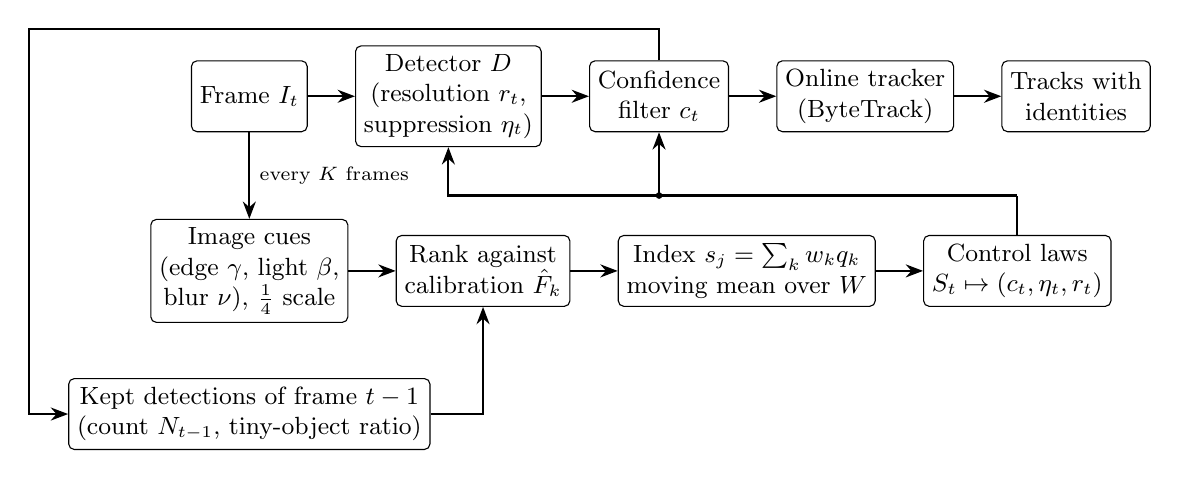
\begin{tikzpicture}[
  node distance=5mm and 6mm,
  box/.style={draw, rounded corners=2pt, align=center, font=\small, minimum height=9mm, inner sep=3pt},
  arr/.style={-{Stealth[length=2.2mm]}, thick}]
\node[box] (frame) {Frame $I_t$};
\node[box, right=of frame] (det) {Detector $D$\\(resolution $r_t$,\\suppression $\eta_t$)};
\node[box, right=of det] (conf) {Confidence\\filter $c_t$};
\node[box, right=of conf] (trk) {Online tracker\\(ByteTrack)};
\node[box, right=of trk] (out) {Tracks with\\identities};
\node[box, below=11mm of frame] (cue) {Image cues\\(edge $\gamma$, light $\beta$,\\blur $\nu$), $\tfrac14$ scale};
\node[box, right=of cue] (rank) {Rank against\\calibration $\hat F_k$};
\node[box, right=of rank] (sci) {Index $s_j=\sum_k w_k q_k$\\moving mean over $W$};
\node[box, right=of sci] (map) {Control laws\\$S_t \mapsto (c_t,\eta_t,r_t)$};
\node[box, below=7mm of cue] (prev) {Kept detections of frame $t-1$\\(count $N_{t-1}$, tiny-object ratio)};
\draw[arr] (frame) -- (det);
\draw[arr] (det) -- (conf);
\draw[arr] (conf) -- (trk);
\draw[arr] (trk) -- (out);
\draw[arr] (frame) -- node[right, font=\scriptsize]{every $K$ frames} (cue);
\draw[arr] (cue) -- (rank);
\draw[arr] (rank) -- (sci);
\draw[arr] (sci) -- (map);
\coordinate (bus) at ($(map.north)+(0,5mm)$);
\draw[thick] (map.north) -- (bus);
\draw[arr] (bus) -| (det.south);
\fill (bus -| conf.south) circle (1.2pt);
\draw[arr] (bus -| conf.south) -- (conf.south);
\draw[arr] (conf.north) -- ++(0,4mm) -| ($(prev.west)+(-5mm,0)$) -- (prev.west);
\draw[arr] (prev.east) -| (rank.south);
\end{tikzpicture}}
\caption{Scene-adaptive operating-point control. The controller runs every $K=10$ frames on a quarter-scale grayscale image and on the detections kept at the previous frame; the chosen operating point is held until the next analysis.}
\label{fig:ch4-system}
\end{figure}

\subsection{Scene cues}
Five cues are computed at each analysis. They were chosen because each targets a failure mode of aerial detection and each costs at most a few image passes on a quarter-resolution frame.

\emph{Crowd.} The number $N_{t-1}$ of detections kept at the previous frame measures density. It is a detector-derived quantity, not a ground-truth count.

\emph{Tiny-object ratio.} The fraction of the previous frame's kept detections whose box area is below $32\times32$ pixels,
\begin{equation}
q_{\mathrm{tiny}} = \frac{1}{N_{t-1}} \sum_{i=1}^{N_{t-1}} \mathbf{1}\left[a_i < 32^2\right],
\label{eq:ch4-tiny}
\end{equation}
with $q_{\mathrm{tiny}}=0$ when $N_{t-1}=0$, measures how much of the scene is at the scale where detectors lose recall \cite{cheng2023smallobject}.

\emph{Edge strength.} The mean Sobel gradient magnitude $\gamma$ of the quarter-scale grayscale image measures texture and clutter.

\emph{Low light.} The mean gray level $\beta$ of the same image measures illumination.

\emph{Blur.} The variance $\nu$ of the Laplacian of the same image is a standard focus measure \cite{pechpacheco2000blur}; low values indicate blur.

\subsection{Label-free calibration}
Raw cue values have incomparable units and dataset-dependent ranges. Each cue is therefore mapped to $[0,1]$ by its empirical distribution function on a calibration set,
\begin{equation}
\hat F_k(x) = \frac{1}{M} \left|\{ m : x_m^{(k)} \le x \}\right|,
\label{eq:ch4-rank}
\end{equation}
where $x_m^{(k)}$, $m=1,\ldots,M$, are the calibration values of cue $k$. The normalized cues are
\begin{equation}
q_{\mathrm{crowd}}=\hat F_{N}(N_{t-1}),\quad q_{\mathrm{edge}}=\hat F_{\gamma}(\gamma),\quad q_{\mathrm{light}}=1-\hat F_{\beta}(\beta),\quad q_{\mathrm{blur}}=1-\hat F_{\nu}(\nu),
\label{eq:ch4-cues}
\end{equation}
and $q_{\mathrm{tiny}}$ is already a fraction. The calibration set contains $M=288$ analysis samples taken every ten frames from the seven VisDrone validation sequences, with image statistics from the frames and crowd counts from the fixed detector run at a single anchor operating point (960 pixels, confidence 0.35, suppression threshold 0.35; person, car, bus, and truck classes). No ground-truth count enters the calibration. On this set the median gray level is 107.6 (interquartile range 85.4--185.1), the median Laplacian variance is 1980, the median gradient magnitude is 66.2, and the median detection count is 10.5 (maximum 41).

The ranking makes the index invariant to monotone rescaling of each cue, and it makes the weights interpretable: a weight multiplies a quantile, not a unit-dependent value. It also means that the index describes a scene relative to the calibration distribution, so that a scene is "complex" if it is more cluttered, darker, blurrier, denser, or has more tiny objects than typical validation scenes.

\subsection{Scene complexity index}
The raw index of analysis $j$ is a convex combination of the normalized cues,
\begin{equation}
s_j = \mathrm{clip}\left(\sum_{k} w_k q_k,\, 0,\, 1\right), \qquad w_k \ge 0,\quad \sum_k w_k = 1,
\label{eq:ch4-sci}
\end{equation}
and the smoothed index is the mean of the last $W$ raw values,
\begin{equation}
S_t = \frac{1}{\min(j,W)} \sum_{i=\max(1,j-W+1)}^{j} s_i, \qquad t \in [\,1+(j-1)K,\; jK\,].
\label{eq:ch4-smooth}
\end{equation}
Analyses occur at frames $t=1, 1+K, 1+2K, \ldots$; between analyses the index and the operating point are held. With $K=10$ and $W=7$, the index at 30 frames per second reflects roughly the last two seconds and changes at most three times per second. The controller state is reset at the start of each sequence.

\section{Analysis of the Scene Complexity Index}\label{sec:ch4-sci}

\subsection{Frozen weights}
Figure~\ref{fig:ch4-sci}a shows the normalized weights of the two frozen profiles, the quality profile Q (trial 24 of the single-objective search) and the balanced profile B (trial 22 of the multi-objective search). Both place the largest weight on edge strength (0.434 for Q and 0.508 for B), a second tier on the tiny-object ratio (0.222 and 0.175) and on crowd density (0.129 and 0.165), and small weights on low light and blur (0.054 and 0.161 for Q; 0.121 and 0.032 for B). The weight on edge strength agrees with the intuition that textured urban scenes are the hard ones for aerial detection. The two searches disagree on blur and low light, which suggests that those cues are weakly identified by seven validation sequences.

\begin{figure}[tbp]
\centering
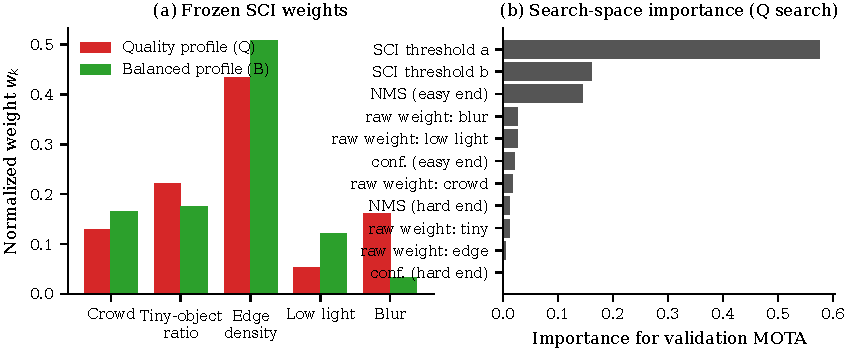
\includegraphics[width=\textwidth]{figures/ch4_fig2_sci_composition.pdf}
\caption{Composition of the scene complexity index. (a) Normalized cue weights of the frozen quality profile Q and balanced profile B. (b) Importance of each search parameter for validation MOTA in the single-objective search that produced Q, as stored with the search record; the two index thresholds dominate.}
\label{fig:ch4-sci}
\end{figure}

\subsection{What the search actually tuned}
The parameter importance scores stored with the single-objective search (Fig.~\ref{fig:ch4-sci}b) are more revealing than the weights. The two thresholds of the resolution rule account for most of the explained variation in validation MOTA (0.575 and 0.161), followed by the easy-end suppression threshold (0.145); every cue weight has importance below 0.03. In other words, the search mostly tuned \emph{how often the controller uses high resolution}, not how the scene is described. The frozen thresholds of Q ($\tau_{\mathrm{m}}=0.135$, $\tau_{\mathrm{h}}=0.287$) are low relative to the typical index, so Q runs at 960 pixels on almost every frame: its mean resolution is 957 pixels on validation and 955 pixels on UAVDT. Its suppression threshold is constant ($\eta_{\mathrm{e}}=\eta_{\mathrm{h}}=0.35$), and only its confidence threshold moves, between 0.30 and 0.40, with a validation mean of 0.341. The optimized quality controller is therefore close to a static operating point at (960, 0.34, 0.35). This observation is the key to the attribution result of Sec.~\ref{sec:ch4-results}.

The balanced profile behaves differently. Its thresholds ($\tau_{\mathrm{m}}=0.293$, $\tau_{\mathrm{h}}=0.666$) place typical scenes in the intermediate and high levels and simple scenes at 512 pixels, giving mean resolutions of 825 pixels on validation, 869 pixels on test-dev, and 829 pixels on UAVDT. Its confidence threshold is constant at 0.40, and its suppression threshold tightens from 0.60 in simple scenes to 0.35 in complex ones (mean 0.47--0.50). Profile B is thus the one that actually switches, and it trades accuracy for fewer identity switches, fewer false positives, and higher throughput.

\subsection{Feedback through the crowd cue}
The crowd and tiny-object cues are computed from detections that already passed the controller's own confidence filter, which closes a loop. In Q the confidence threshold rises with the index; a higher index therefore removes low-scoring boxes, lowers the next crowd count, and pulls the index back down. This is negative feedback, which keeps the operating point stable. The hand-designed controller of Sec.~\ref{sec:ch4-control} lowers the confidence threshold as the index rises, which admits more boxes and raises the next crowd count: positive feedback, bounded only by the clipping of its thresholds. The moving mean of Eq.~\eqref{eq:ch4-smooth} and the ten-frame stride damp both loops. The analysis does not change any result, but it explains why the validation search preferred a controller whose confidence threshold increases with complexity.

\section{Adaptive Control Strategy}\label{sec:ch4-control}

\subsection{Calibrated control laws}
The calibrated controller maps the smoothed index to the operating point by two linear laws and one piecewise-constant law:
\begin{align}
c_t &= c_{\mathrm{e}} + S_t\,(c_{\mathrm{h}} - c_{\mathrm{e}}), \label{eq:ch4-conf}\\
\eta_t &= \eta_{\mathrm{e}} + S_t\,(\eta_{\mathrm{h}} - \eta_{\mathrm{e}}), \label{eq:ch4-nms}\\
r_t &= \begin{cases} r_0, & S_t < \tau_{\mathrm{m}},\\ r_1, & \tau_{\mathrm{m}} \le S_t < \tau_{\mathrm{h}},\\ r_2, & S_t \ge \tau_{\mathrm{h}}, \end{cases} \label{eq:ch4-res}
\end{align}
with resolution levels $(r_0, r_1, r_2) = (512, 928, 960)$ pixels. The eleven parameters are the five weights, the four endpoints $c_{\mathrm{e}}, c_{\mathrm{h}}, \eta_{\mathrm{e}}, \eta_{\mathrm{h}}$, and the two thresholds $\tau_{\mathrm{m}}, \tau_{\mathrm{h}}$. Figure~\ref{fig:ch4-map} plots the three laws for both profiles, and Table~\ref{tab:ch4-settings} lists all frozen configurations.

\begin{figure}[tbp]
\centering
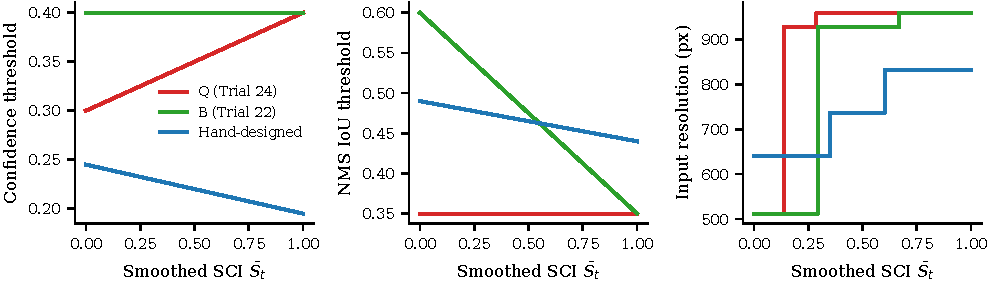
\includegraphics[width=\textwidth]{figures/ch4_fig3_adaptation_map.pdf}
\caption{Adaptation maps: confidence threshold, suppression threshold, and input resolution as functions of the smoothed index for the quality profile Q, the balanced profile B, and the hand-designed controller (scene-label adjustments of the hand-designed controller omitted).}
\label{fig:ch4-map}
\end{figure}

\begin{table}[tbp]
\centering
\caption{Frozen configurations compared in this study. Confidence and NMS entries give the value at $S=0$ and at $S=1$ (linear in between); resolution is the long-side input size in pixels. All adaptive controllers analyze every $K=10$ frames with a moving mean over $W=7$ analyses.}
\label{tab:ch4-settings}
\small\setlength{\tabcolsep}{4pt}
\begin{adjustbox}{max width=\textwidth}
\begin{tabular}{>{\raggedright\arraybackslash}p{3.3cm}>{\raggedright\arraybackslash}p{3.0cm}>{\raggedright\arraybackslash}p{3.0cm}>{\raggedright\arraybackslash}p{3.8cm}>{\raggedright\arraybackslash}p{1.4cm}}
\hline
Configuration & Confidence & NMS IoU & Resolution & Tracker \\
\hline
Static default & 0.25 & 0.45 & 640 & default \\
Hand-designed controller & $0.245-0.05S$, clipped to 0.19--0.28 & $0.49-0.05S$, clipped to 0.40--0.52 & 640/736/832 (rules in Sec.~\ref{sec:ch4-control}) & tuned \\
Quality profile Q (trial 24) & 0.30$\to$0.40 & 0.35$\to$0.35 & 512/928/960 at $S\ge0.135/0.287$ & tuned \\
Balanced profile B (trial 22) & 0.40$\to$0.40 & 0.60$\to$0.35 & 512/928/960 at $S\ge0.293/0.666$ & tuned \\
Matched static anchor & 0.35 & 0.35 & 960 & tuned \\
\hline
\multicolumn{5}{l}{Tracker profiles (ByteTrack): default = high 0.25, low 0.10, new 0.25, buffer 30, match 0.80;}\\
\multicolumn{5}{l}{tuned = high 0.18, low 0.04, new 0.20, buffer 45, match 0.86.}\\
\hline
\end{tabular}
\end{adjustbox}
\end{table}


\subsection{Hand-designed controller}
The hand-designed controller is the earlier version of the same idea and serves as the adaptive baseline. Its index uses fixed saturating transforms instead of calibrated ranks:
\begin{equation}
\begin{split}
s_j = \mathrm{clip}\Big(&0.30\min\left(\tfrac{N_{t-1}}{30},1\right) + 0.20\min\left(\tfrac{e}{0.14},1\right) + 0.30\,q_{\mathrm{tiny}}\\
&+ 0.10\,\mathbf{1}[\beta<80] + 0.05\,\mathbf{1}[\nu<180],\;0,\;1\Big),
\end{split}
\label{eq:ch4-heur}
\end{equation}
where $e$ is the fraction of Canny edge pixels of the quarter-scale image. It also assigns a scene label (night, blur, tiny, crowded, or clear) from the same cues. Its confidence threshold $0.245-0.05S_t$ decreases with complexity, is lowered by a further 0.012 in crowded, tiny, or night scenes, and is clipped to $[0.19, 0.28]$; its suppression threshold $0.49-0.05S_t$ is lowered by 0.012 in blurred scenes and clipped to $[0.40, 0.52]$. Its resolution is 832 pixels when $S_t>0.60$ or the tiny-object ratio exceeds 0.5, 736 pixels when $S_t>0.35$ or the scene is labelled crowded or tiny, and 640 pixels otherwise. It uses the same analysis stride and smoothing window as the calibrated controller ($K=10$, $W=7$).

The two controllers encode opposite hypotheses about confidence. The hand-designed controller is recall-oriented: in hard scenes it admits weaker boxes. The calibrated profiles are precision-oriented: Q raises the confidence threshold in hard scenes, and B holds it at 0.40 while tightening suppression. The validation evidence of Sec.~\ref{sec:ch4-ablation} favors the precision-oriented choice for this detector and tracker.

\subsection{Update schedule and cost}
All controllers analyze the first frame of each sequence and every tenth frame thereafter; the image cues require one resize, one color conversion, two Sobel filters, and one Laplacian on a quarter-scale image, and the detection cues reuse boxes that the tracker already holds. In the matched static run on test-dev, where the controller code path ran without cue analysis, the per-frame controller time was 0.005 ms against 19.5 ms for the detector and 3.6 ms for the tracker. The cue analysis cost of the adaptive runs was not profiled separately; it is included in their end-to-end processing throughput.

\section{Detection and Tracking Pipeline}\label{sec:ch4-pipeline}

\subsection{Detector}
The detector is the Ultralytics YOLOv8n model pretrained on the COCO dataset (Ultralytics library version 8.3.200), run in half precision through PyTorch on one NVIDIA Tesla T4 graphics processor with at most 1000 detections per frame. Only the person, car, bus, and truck classes are kept on VisDrone; car, bus, and truck are kept on UAVDT, whose annotations cover vehicles only. The detector is not fine-tuned on aerial data, which keeps the controller evaluation independent of any training choice but also bounds the absolute accuracy (Sec.~\ref{sec:ch4-limits}).

\subsection{Tracker}
The tracker is the Ultralytics implementation of ByteTrack \cite{zhang2022bytetrack} with score fusion and a nominal frame rate of 30. Two profiles are used (Table~\ref{tab:ch4-settings}): the library-style default profile (high threshold 0.25, low threshold 0.10, new-track threshold 0.25, buffer 30 frames, matching threshold 0.80) and a tuned profile selected in earlier validation work (0.18, 0.04, 0.20, 45 frames, 0.86). The tuned profile is part of every adaptive system and of the matched static anchor; the static default uses the default profile.

One interaction between detector and tracker needs to be stated explicitly. Detections below the controller's confidence threshold are removed before the tracker. Because every confidence threshold used in this study (0.19 or higher) is at or above the tracker's high threshold, every detection reaching the tracker counts as high-confidence, and all of them except boxes of the hand-designed controller scored between 0.19 and 0.20 are eligible to start a new track. ByteTrack's second association stage, which recovers occluded objects from low-confidence boxes, therefore receives no input in these configurations. The tuned profile acts mainly through its longer buffer and its looser matching threshold.

\subsection{Timing protocol}
Throughput is reported as processing frames per second: the number of frames divided by the summed per-frame time of cue analysis, detection (with device synchronization), and tracking. Frames are decoded from JPEG files before timing, and all resolutions a system can request are warmed up before the first timed frame. Decoding is excluded because an onboard pipeline receives decoded frames from the camera. In the matched static run, decoding cost 22.5 ms per frame on average, and throughput including decoding was 21.90 frames per second, below the 25 frames-per-second target. The throughput figures of this chapter are therefore processing throughput on already-decoded frames, not end-to-end real-time performance on board. The gate of 25 frames per second was applied to the whole-split processing throughput.

\section{Experimental Setup}\label{sec:ch4-setup}

\subsection{Data}
Table~\ref{tab:ch4-data} lists the data. All design decisions used the seven sequences of the VisDrone2019 multi-object tracking validation split \cite{zhu2022visdrone}. The seventeen sequences of the test-dev split were held out until a locked three-system comparison. The twenty sequences of the UAVDT test split \cite{du2018uavdt} were used once, as a zero-tuning cross-dataset test.

\begin{table}[tbp]
\centering
\caption{Data splits and their role. No test sequence was used for any selection, calibration, or tuning decision.}
\label{tab:ch4-data}
\small\setlength{\tabcolsep}{4pt}
\begin{adjustbox}{max width=\textwidth}
\begin{tabular}{llrrl}
\hline
Dataset & Split & Sequences & Frames & Role \\
\hline
VisDrone2019-MOT & validation & 7 & 2,846 & cue calibration, sweeps, ablations, optimization \\
VisDrone2019-MOT & test-dev & 17 & 6,635 & locked held-out comparison \\
UAVDT & test & 20 & 16,592 & zero-tuning cross-dataset test \\
\hline
\end{tabular}
\end{adjustbox}
\end{table}


\subsection{Evaluation protocol}
Evaluation is class-agnostic. On VisDrone, ground-truth boxes of the pedestrian, car, van, truck, and bus categories are kept when they are marked as considered, with occlusion and truncation levels below 2; all detector classes are pooled. This is a research protocol, not the official VisDrone evaluation, so the absolute numbers are not comparable with the VisDrone leaderboard. On UAVDT, a frozen adapter (checked by a self-test on a training sequence, which it reproduced with perfect scores) removes ground truth marked out of scope, normalizes identities, removes predictions strictly contained in ignore regions for the eighteen sequences that provide them, and matches at an overlap of 0.5. All metrics were computed with the TrackEval library pinned to commit 12c8791.

HOTA is the primary metric because it weighs detection and association equally \cite{luiten2021hota}; MOTA, IDF1, identity switches, false negatives, and false positives are reported alongside. Uncertainty is quantified by a paired bootstrap over sequences \cite{efron1993bootstrap}: sequences are resampled with replacement 5,000 times (seed 42), the metric difference between two systems is recomputed on each resample from the pooled counts, and the 2.5th and 97.5th percentiles form the 95\% interval. A win, tie, or loss count per sequence is reported as a complementary, distribution-free summary.

\subsection{Selection chain}
The selection chain used the validation split only.

\emph{Operating-point sweeps.} With the tuned tracker, three one-at-a-time sweeps measured validation accuracy and throughput for resolutions from 512 to 960 pixels in steps of 32, confidence thresholds from 0.05 to 0.50, and suppression thresholds from 0.30 to 0.80. Confidence and suppression values were kept if they met the throughput gate and at least the reference accuracy of the sweep, which retained confidence values 0.25--0.45 and suppression values 0.30--0.70. Three resolution levels were retained by a predeclared rule: a low-compute feasible level, the highest-quality feasible level, and the highest-quality distinct intermediate level, which gave 512, 960, and 928 pixels.

\emph{Temporal settings.} A grid of smoothing windows $W\in\{1,3,5,7,9\}$ and analysis strides $K\in\{1,5,10,15,20\}$ was evaluated with the hand-designed controller, and $W=7$, $K=10$ was frozen.

\emph{Quality profile.} A tree-structured Parzen estimator search of at most 50 trials explored the five raw weights (normalized to sum to one), the confidence and suppression endpoints within the retained sets, and the two resolution thresholds. The selection rule, fixed before the search, required the throughput gate and no more identity switches than the hand-designed controller on validation (271), and then selected the highest MOTA, breaking ties by fewer identity switches, then HOTA, IDF1, and throughput. Trial 24 was selected, with validation HOTA 36.11\%, MOTA 23.04\%, IDF1 40.76\%, 270 identity switches, and 37.17 frames per second.

\emph{Balanced profile.} A second, multi-objective search (seed 42) maximized MOTA and minimized identity switches with only the throughput gate. Of 50 planned trials, 49 completed. The Pareto front ranged from trial 16 (MOTA 22.83\%, 308 switches) to trial 8 (11.54\%, 114 switches). A balanced score, declared before the search, averaged min--max normalized MOTA and normalized identity-switch reduction, and it selected trial 22 (validation MOTA 19.33\%, HOTA 31.65\%, 168 switches, 51.41 frames per second).

\subsection{Held-out protocol}
Before the test split was opened, a protocol file fixed the three compared systems (static default, hand-designed controller, quality profile Q), their configuration hashes, the calibration hash, the ground-truth filter, the evaluator commit, the throughput gate, and the requirement of a T4 processor. Each system ran as a separate worker in its own session and wrote an immutable result file; the merge step refused to run until all three existed. The quality-profile worker resumed from per-sequence checkpoints after an interruption, with no parameter change. The balanced profile was frozen after its selection and tested with the same machinery; its first test attempt was interrupted before any result was saved, and an exact technical rerun of the frozen configuration produced the reported result. The UAVDT test was run for the static default and both frozen profiles under a separate lock that forbade any tuning, recalibration, or selection on UAVDT.

After these tests were complete, the matched static anchor (960 pixels, confidence 0.35, suppression 0.35, tuned tracker, no adaptation) was evaluated on test-dev and paired with the quality profile. It was not part of the preregistered comparison: it serves only to attribute the measured gain, and its throughput was measured in a separate session.

\section{Main Results}\label{sec:ch4-results}

\subsection{Held-out test-dev}
Table~\ref{tab:ch4-main} gives the held-out results and Table~\ref{tab:ch4-boot} the paired bootstrap intervals.

\begin{table}[tbp]
\centering
\caption{Held-out results (percent for HOTA, MOTA, IDF1; counts for IDS, FN, FP; processing frames per second on one NVIDIA Tesla T4, each system measured in its own session). No entry is marked as best because the profiles target different trade-offs.}
\label{tab:ch4-main}
\small\setlength{\tabcolsep}{4pt}
\begin{adjustbox}{max width=\textwidth}
\begin{tabular}{lrrrrrrr}
\hline
System & HOTA & MOTA & IDF1 & IDS & FN & FP & FPS \\
\hline
\multicolumn{8}{l}{\textit{VisDrone2019-MOT test-dev (17 sequences, 6,635 frames)}}\\
Static default & 28.43 & 19.73 & 32.72 & 1235 & 155051 & 16308 & 36.53 \\
Hand-designed controller & 32.70 & 23.24 & 39.52 & 1061 & 138967 & 25025 & 41.96 \\
Quality profile Q & 33.84 & 26.95 & 41.55 & 1184 & 136858 & 19029 & 38.98 \\
Balanced profile B & 31.22 & 23.79 & 37.87 & 919 & 149307 & 13632 & 46.02 \\
Matched static anchor & 33.93 & 27.00 & 41.77 & 1197 & 136391 & 19374 & 43.23$^{a}$ \\
\multicolumn{8}{l}{\textit{UAVDT test (20 sequences, 16,592 frames), no tuning on UAVDT}}\\
Static default & 24.08 & 13.84 & 27.89 & 558 & 270189 & 22974 & 65.01 \\
Quality profile Q & 28.39 & 17.40 & 34.45 & 321 & 258376 & 22896 & 58.35 \\
Balanced profile B & 26.93 & 16.12 & 32.01 & 308 & 266894 & 18758 & 61.46 \\
\hline
\multicolumn{8}{l}{$^{a}$Run after the freeze for attribution only; frames per second measured in a separate T4 session.}\\
\hline
\end{tabular}
\end{adjustbox}
\end{table}


\begin{sidewaystable}
\centering
\caption{Paired sequence-level bootstrap (5,000 resamples, seed 42): observed difference and 95\% percentile interval. HOTA, MOTA and IDF1 in percentage points; IDS reduction in switches (positive = fewer switches for the first system).}
\label{tab:ch4-boot}
\small\setlength{\tabcolsep}{4pt}
\begin{adjustbox}{max width=\textheight}
\begin{tabular}{llllll}
\hline
Data & Comparison & $\Delta$HOTA & $\Delta$MOTA & $\Delta$IDF1 & IDS reduction \\
\hline
VisDrone & Q vs static default & $+5.41$ [$+4.13$, $+6.90$] & $+7.22$ [$+5.44$, $+9.29$] & $+8.82$ [$+6.90$, $+11.05$] & $+51$ [$-114$, $+219$] \\
VisDrone & Q vs hand-designed & $+1.14$ [$+0.14$, $+2.27$] & $+3.71$ [$+2.39$, $+5.19$] & $+2.03$ [$+0.59$, $+3.77$] & $-123$ [$-244$, $-14$] \\
VisDrone & Q vs matched static anchor & $-0.09$ [$-0.25$, $+0.06$] & $-0.05$ [$-0.25$, $+0.16$] & $-0.23$ [$-0.50$, $+0.02$] & $+13$ [$-23$, $+46$] \\
VisDrone & B vs static default & $+2.79$ [$+0.75$, $+4.66$] & $+4.06$ [$+0.95$, $+6.89$] & $+5.15$ [$+2.03$, $+8.08$] & $+316$ [$+175$, $+470$] \\
VisDrone & B vs Q & $-2.62$ [$-4.00$, $-1.69$] & $-3.16$ [$-6.14$, $-1.35$] & $-3.68$ [$-5.88$, $-2.24$] & $+265$ [$+82$, $+502$] \\
UAVDT & Q vs static default & $+4.30$ [$+2.74$, $+5.71$] & $+3.56$ [$+1.45$, $+5.81$] & $+6.57$ [$+3.81$, $+8.82$] & $+237$ [$+104$, $+377$] \\
UAVDT & B vs static default & $+2.85$ [$+1.24$, $+4.35$] & $+2.28$ [$+0.72$, $+4.16$] & $+4.13$ [$+1.63$, $+6.49$] & $+250$ [$+110$, $+404$] \\
UAVDT & B vs Q & $-1.46$ [$-2.19$, $-0.91$] & $-1.28$ [$-2.44$, $-0.20$] & $-2.44$ [$-3.74$, $-1.37$] & $+13$ [$-20$, $+50$] \\
\hline
\end{tabular}
\end{adjustbox}
\end{sidewaystable}


Against the static default, the quality profile raised HOTA from 28.43\% to 33.84\% ($\Delta=+5.41$, 95\% interval $[+4.13, +6.90]$), MOTA by 7.22 points, and IDF1 by 8.82 points, and it won on all 17 sequences. The gain comes mostly from recall: false negatives fell by 18,193, while false positives rose by 2,721. Identity switches fell by 51, but that interval includes zero. Throughput was 38.98 frames per second against 36.53 for the default, both above the gate.

Against the hand-designed controller, the quality profile gained 1.14 HOTA points ($[+0.14, +2.27]$), 3.71 MOTA points, and 2.03 IDF1 points, and it won on 13 of 17 sequences. It produced 5,996 fewer false positives and 2,109 fewer false negatives, but 123 more identity switches, and that difference is significant ($[-244, -14]$ in switch reduction). The hand-designed controller therefore remains the identity-switch leader of the preregistered comparison, and the quality profile is not better on every metric.

The balanced profile sits at a different point of the trade-off. On test-dev it had the fewest identity switches (919), the fewest false positives (13,632), and the highest throughput (46.02 frames per second), with HOTA 31.22\%. It was significantly better than the static default on every metric, including 316 fewer identity switches ($[+175, +470]$), and significantly worse than the quality profile in HOTA ($-2.62$), MOTA, and IDF1, while having 265 fewer switches ($[+82, +502]$).

\subsection{Cross-dataset test without tuning}
On UAVDT, no parameter was changed. The quality profile raised HOTA from 24.08\% to 28.39\% ($[+2.74, +5.71]$), MOTA by 3.56 points, and IDF1 by 6.57 points, and it reduced identity switches from 558 to 321 ($[+104, +377]$), winning 15 of 20 sequences with 2 ties and 3 losses. The balanced profile improved over the default by 2.85 HOTA points ($[+1.24, +4.35]$) with 250 fewer switches, but it was significantly below the quality profile in HOTA ($-1.46$), MOTA, and IDF1, and its 13-switch advantage over the quality profile is not significant ($[-20, +50]$). Both profiles ran slower than the static default on UAVDT (58.35 and 61.46 against 65.01 frames per second), because both use higher mean resolutions than the default's 640 pixels.

Across both datasets, the quality profile is the accuracy leader of the frozen systems, and the balanced profile is a reproducible identity, false-positive, and throughput trade-off on VisDrone whose identity advantage over the quality profile does not transfer significantly to UAVDT.

\subsection{Attribution: the matched static anchor}
The quality profile runs at the top resolution on almost every frame with a confidence threshold near 0.34 and a constant suppression threshold of 0.35 (Sec.~\ref{sec:ch4-sci}). Its natural control is therefore the static operating point (960, 0.35, 0.35) with the same tuned tracker, which is also the anchor of the cue calibration. On validation, that anchor reached 36.08\% HOTA against 36.11\% for the full quality profile (Table~\ref{tab:ch4-ablation}). On test-dev, the anchor reached 33.93\% HOTA against 33.84\% for the quality profile: $\Delta=-0.09$ for the profile, with interval $[-0.25, +0.06]$ (Table~\ref{tab:ch4-boot}). MOTA, IDF1, and identity switches likewise differ by amounts whose intervals include zero.

On validation, the two parts of that configuration can be separated with the ablation runs of Table~\ref{tab:ch4-ablation}: at the default operating point, the tuned tracker profile added 1.03 HOTA points (H0 to H1), and moving the detector to the anchor operating point with the same tracker added a further 5.21 points (H1 to C0). Most of the calibration gain therefore comes from the detector operating point, and a smaller part from the tracker profile; this decomposition is a validation result, because the tracker profiles were not separated on the held-out splits.

The held-out gains of the quality profile over the static default (+5.41 HOTA) and over the hand-designed controller (+1.14) are therefore attributable to the validation-calibrated operating point, namely high resolution, a precision-oriented confidence threshold, a tight suppression threshold, and the tuned tracker profile, and not to frame-to-frame switching. The frozen protocol and the post hoc anchor jointly support that conclusion; the anchor was not available as a preregistered competitor, which is why it is reported as an attribution analysis rather than as a fourth system of the locked comparison.

\subsection{Validation-to-test transfer}
All selection used seven validation sequences, and the controller has eleven parameters, so overfitting to the validation split is a natural concern. Three observations bound it. First, the gain of the quality profile over the static default was 6.27 HOTA points on validation (36.11 against 29.84 percent, Table~\ref{tab:ch4-ablation}), 5.41 points on the seventeen held-out test-dev sequences, and 4.30 points on UAVDT without any retuning, so most of the validation gain transferred to unseen sequences and to a second dataset. Second, the search concentrated its effect on the two resolution thresholds (Sec.~\ref{sec:ch4-sci}), and the selected controller behaves like a static operating point with three parameters, which is the configuration that the matched static anchor reproduces. Third, the one constraint that did not transfer, the identity-switch bound, is reported as a failure in Sec.~\ref{sec:ch4-failure}. The transfer supports the calibrated operating point; it does not show that the eleven parameters are individually identified, and the weakly identified cue weights (Sec.~\ref{sec:ch4-sci}) should not be read as a general ranking of scene cues.

\subsection{Per-sequence behavior}
Figure~\ref{fig:ch4-perseq} shows the per-sequence HOTA differences. On test-dev, the gain of the quality profile over the default is positive everywhere and ranges from +1.07 to +13.10 points; the largest gain occurs on the sequence where all systems are weakest (default HOTA 7.10\%). Against the hand-designed controller, four sequences are losses, the largest by 4.69 points. On UAVDT, the gains of both profiles are positive on most sequences, with a tail of losses discussed in Sec.~\ref{sec:ch4-failure}.

\begin{figure}[tbp]
\centering
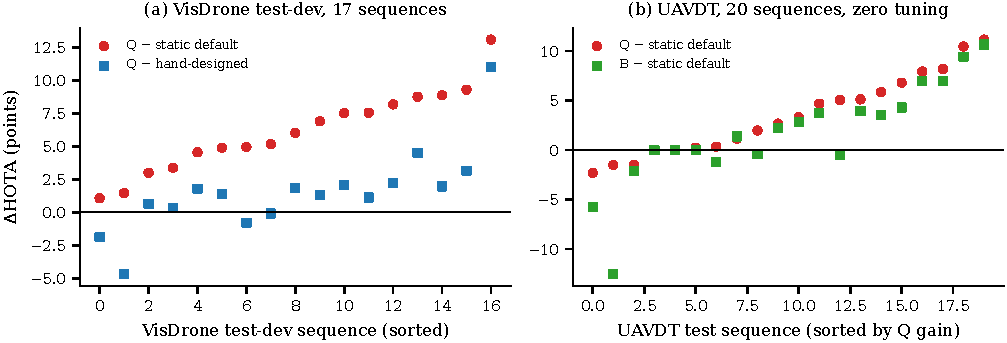
\includegraphics[width=\textwidth]{figures/ch4_fig6_per_sequence.pdf}
\caption{Per-sequence HOTA differences, sorted. (a) VisDrone test-dev: quality profile minus static default and minus the hand-designed controller. (b) UAVDT: quality and balanced profiles minus static default, without any tuning on UAVDT.}
\label{fig:ch4-perseq}
\end{figure}

\section{Ablation}\label{sec:ch4-ablation}
Table~\ref{tab:ch4-ablation} and Fig.~\ref{fig:ch4-ablation} decompose both controllers on the validation split.

\begin{table}[tbp]
\centering
\caption{Component ablations on VisDrone2019-MOT validation (7 sequences). FPS is processing throughput on a T4; mean resolution, confidence and NMS are averaged over frames.}
\label{tab:ch4-ablation}
\small\setlength{\tabcolsep}{4pt}
\begin{adjustbox}{max width=\textwidth}
\begin{tabular}{llrrrrrrrr}
\hline
Stage & Components & HOTA & MOTA & IDF1 & IDS & FPS & Res. & Conf. & NMS \\
\hline
\multicolumn{10}{l}{\textit{Hand-designed controller}}\\
H0 & static default, default tracker & 29.84 & 17.63 & 30.89 & 283 & 44.1 & 640 & 0.250 & 0.450 \\
H1 & + tuned tracker & 30.86 & 17.80 & 32.85 & 217 & 44.5 & 640 & 0.250 & 0.450 \\
H2 & + adaptive conf./NMS (640 px) & 31.38 & 17.64 & 33.73 & 210 & 40.7 & 640 & 0.218 & 0.474 \\
H2R & tuned tracker + adaptive resolution only & 32.45 & 18.42 & 35.67 & 241 & 39.6 & 722 & 0.250 & 0.450 \\
H3 & full hand-designed controller & 33.06 & 18.16 & 36.30 & 271 & 38.0 & 725 & 0.218 & 0.474 \\
\multicolumn{10}{l}{\textit{Optimized controller (quality profile Q)}}\\
C0 & static anchor 960/0.35/0.35, tuned tracker & 36.08 & 23.08 & 40.60 & 266 & 37.9 & 960 & 0.350 & 0.350 \\
C1 & + adaptive confidence & 36.11 & 23.01 & 40.73 & 271 & 35.3 & 960 & 0.341 & 0.350 \\
C2 & + adaptive NMS & 36.11 & 23.01 & 40.73 & 271 & 35.5 & 960 & 0.341 & 0.350 \\
C3 & + adaptive resolution (full Q) & 36.11 & 23.04 & 40.76 & 270 & 35.4 & 957 & 0.341 & 0.350 \\
\hline
\end{tabular}
\end{adjustbox}
\end{table}


\begin{figure}[tbp]
\centering
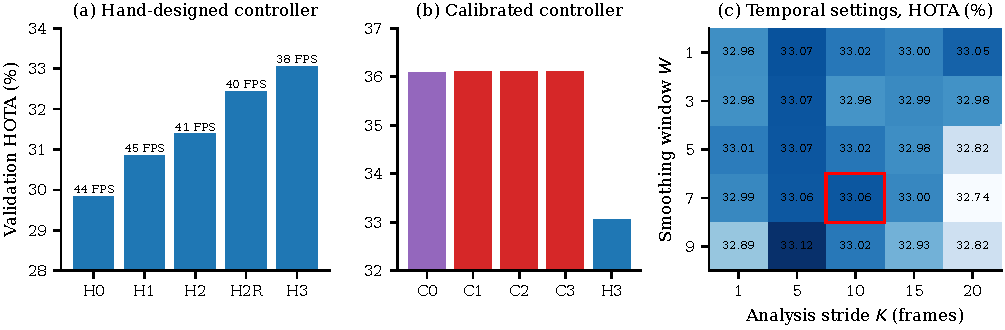
\includegraphics[width=\textwidth]{figures/ch4_fig5_ablation.pdf}
\caption{Validation ablations. (a) Hand-designed controller: H0 static default with default tracker; H1 tuned tracker; H2 adaptive confidence and suppression at 640 pixels; H2R adaptive resolution only; H3 full controller. (b) Calibrated controller: C0 static anchor; C1 adaptive confidence; C2 adaptive confidence and suppression; C3 full quality profile; H3 shown for reference. (c) Temporal grid of the hand-designed controller, selected setting outlined.}
\label{fig:ch4-ablation}
\end{figure}

\subsection{Hand-designed controller}
Starting from the static default (H0, 29.84\% HOTA), tuning the tracker (H1) added 1.03 HOTA points and removed 66 identity switches at unchanged throughput. Adaptive confidence and suppression at a fixed 640 pixels (H2) added a further 0.52 points. Adaptive resolution alone, with static confidence and suppression (H2R), reached 32.45\%, 1.59 points above H1, at a mean resolution of 722 pixels. The full controller (H3) reached 33.06\%, 2.20 points above H1, at 38.0 frames per second against 44.5 for H1. For the hand-designed controller, therefore, scene-driven switching does add accuracy, and most of it comes from resolution. The operating range of that controller is narrow and low (640--832 pixels), and its adaptive resolution moves the operating point into the range where accuracy grows fastest with resolution (Table~\ref{tab:ch4-speed}).

\subsection{Calibrated controller}
For the quality profile the picture is different. The static anchor (C0) already reached 36.08\% HOTA, 3.01 points above the full hand-designed controller. Adding adaptive confidence (C1) changed HOTA by +0.03 points and identity switches by +5. Adding adaptive suppression (C2) changed nothing, as expected, because the profile's two suppression endpoints are equal; the identical metrics confirm that the ablation machinery isolates components exactly. Adding adaptive resolution (C3) changed HOTA by less than 0.01 points, because the index almost never falls below the resolution thresholds. The components of the calibrated controller are therefore measurable but negligible, which the held-out anchor comparison of Sec.~\ref{sec:ch4-results} confirms on unseen data.

\subsection{Temporal settings}
Across the 25 temporal settings, HOTA of the hand-designed controller varied only between 32.74\% and 33.12\% (Table~\ref{tab:ch4-temporal}); the frozen setting $W=7$, $K=10$ gave 33.06\%. Analyzing every frame ($K=1$) cost 6 to 14 frames per second relative to $K\ge5$ in the same grid without an accuracy benefit, so infrequent analysis is the right design for this controller. Temporal parameters are second-order for accuracy and first-order for cost.

\begin{table}[tbp]
\centering
\caption{Temporal settings of the hand-designed controller on VisDrone2019-MOT validation: HOTA (\%) / processing FPS for smoothing window $W$ (analyses) and analysis stride $K$ (frames). The selected setting is $W=7$, $K=10$.}
\label{tab:ch4-temporal}
\small\setlength{\tabcolsep}{4pt}
\begin{adjustbox}{max width=\textwidth}
\begin{tabular}{rccccc}
\hline
$W$ \textbackslash{} $K$ & 1 & 5 & 10 & 15 & 20 \\
\hline
1 & 32.98 / 34.3 & 33.07 / 45.3 & 33.02 / 45.9 & 33.00 / 47.3 & 33.05 / 47.9 \\
3 & 32.98 / 37.0 & 33.07 / 46.8 & 32.98 / 47.8 & 32.99 / 48.9 & 32.98 / 48.1 \\
5 & 33.01 / 36.1 & 33.07 / 45.7 & 33.02 / 48.1 & 32.98 / 48.7 & 32.82 / 49.0 \\
7 & 32.99 / 36.0 & 33.06 / 45.8 & \textbf{33.06 / 43.9} & 33.00 / 48.5 & 32.74 / 49.8 \\
9 & 32.89 / 37.3 & 33.12 / 47.8 & 33.02 / 48.3 & 32.93 / 43.5 & 32.82 / 45.1 \\
\hline
\end{tabular}
\end{adjustbox}
\end{table}


\section{Accuracy--Runtime Analysis}\label{sec:ch4-runtime}
Figure~\ref{fig:ch4-runtime} and Table~\ref{tab:ch4-speed} relate accuracy and throughput.

\begin{figure}[tbp]
\centering
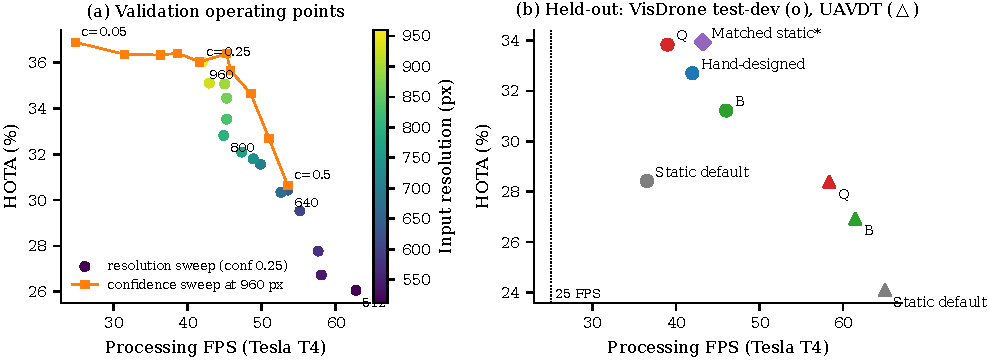
\includegraphics[width=\textwidth]{figures/ch4_fig4_accuracy_runtime.pdf}
\caption{Accuracy versus processing throughput on one Tesla T4. (a) Validation operating points: resolution sweep at confidence 0.25 and confidence sweep at 960 pixels. (b) Held-out systems on VisDrone test-dev (circles) and UAVDT (triangles); the matched static anchor (diamond) was timed in a separate session. The dotted line marks 25 frames per second.}
\label{fig:ch4-runtime}
\end{figure}

\begin{table}[tbp]
\centering
\caption{Accuracy--throughput trade-off of the detector input resolution on VisDrone2019-MOT validation (confidence 0.25, NMS IoU 0.70, tuned tracker; T4 processing throughput and 95th-percentile per-frame latency).}
\label{tab:ch4-speed}
\small\setlength{\tabcolsep}{4pt}
\begin{adjustbox}{max width=\textwidth}
\begin{tabular}{rrrrrrr}
\hline
Resolution & HOTA & MOTA & IDF1 & IDS & FPS & P95 latency (ms) \\
\hline
512 & 26.05 & 13.93 & 26.00 & 216 & 62.7 & 26.1 \\
576 & 27.77 & 15.67 & 29.19 & 240 & 57.6 & 29.0 \\
640 & 30.43 & 16.96 & 32.23 & 326 & 53.5 & 32.1 \\
704 & 31.56 & 17.35 & 34.26 & 322 & 49.8 & 33.6 \\
768 & 32.09 & 18.15 & 34.45 & 359 & 47.3 & 36.9 \\
832 & 33.53 & 18.92 & 37.02 & 413 & 45.3 & 37.5 \\
896 & 35.07 & 20.17 & 39.08 & 399 & 45.0 & 38.2 \\
928 & 35.10 & 20.67 & 39.70 & 416 & 42.9 & 38.6 \\
960 & 36.03 & 20.87 & 40.25 & 420 & 42.0 & 40.9 \\
\hline
\end{tabular}
\end{adjustbox}
\end{table}


\subsection{Resolution dominates both accuracy and cost}
In the validation sweep, raising the input resolution from 512 to 960 pixels raised HOTA from 26.05\% to 36.03\% and lowered throughput from 62.7 to 42.0 frames per second, with the 95th-percentile per-frame latency growing from 26.1 to 40.9 ms. The confidence threshold mostly moves the balance between false positives and false negatives: at 960 pixels, HOTA stayed within 36.9\% and 35.6\% for thresholds between 0.05 and 0.35 and fell to 30.6\% at 0.50, while false positives fell from 18,056 to 3,426. The very low thresholds cost throughput through the tracker (24.8 frames per second at 0.05), which is why they failed the gate. The suppression threshold had almost no effect between 0.30 and 0.55 and hurt identity switches above 0.60 (266 switches at 0.30--0.50, 467 at 0.80). The calibrated profiles lie close to the best sweep points, which is consistent with the finding that their benefit is the operating point itself.

\subsection{Held-out throughput}
All held-out systems met the gate on the whole split, and every individual test-dev sequence was processed above 25 frames per second by every system (the slowest sequence of the quality profile ran at 27.5). The balanced profile was the fastest adaptive system (46.02 frames per second on test-dev), because it spends part of the time at 512 pixels.

\subsection{Measurement variability}
Throughput measured in separate sessions on the same processor class varies more than the differences between some systems. The static anchor configuration was timed at 37.92 frames per second in the component ablation and at 44.78 in the suppression sweep, with identical tracking metrics. The full hand-designed controller was timed at 37.96, 42.09, and 43.95 frames per second in three validation runs of the same configuration. Throughput differences of a few frames per second between systems measured in different sessions, including the 2.97 frames-per-second difference between the quality profile and the hand-designed controller on test-dev, should therefore not be interpreted as algorithmic differences. The accuracy metrics are unaffected by this variability.

\section{Failure Analysis}\label{sec:ch4-failure}

\subsection{Identity switches}
The largest failure of the quality profile is identity fragmentation relative to the hand-designed controller on test-dev (123 more switches, significant). On validation the two were matched by construction (270 against 271 switches), so the constraint of Eq.~\eqref{eq:ch4-objective} did not transfer. A plausible mechanism is the tracker interaction of Sec.~\ref{sec:ch4-pipeline}: with a precision-oriented confidence threshold, boxes that briefly drop below the threshold disappear from the tracker entirely, and ByteTrack's low-score recovery cannot bridge them. The balanced profile, which optimized identity switches directly, did control them on both datasets.

\subsection{Sequences where adaptation loses}
Against the hand-designed controller, the quality profile lost on four of the 17 test-dev sequences by 0.10, 0.79, 1.87, and 4.69 HOTA points. On UAVDT, the quality profile lost to the static default on three of 20 sequences, by 1.48 to 2.29 points. The balanced profile's worst UAVDT sequence lost 12.52 points against the default, with false negatives rising from 3,477 to 4,256: its fixed confidence threshold of 0.40 removes true detections that the default's 0.25 keeps. A fixed precision-oriented threshold is therefore a risk under a domain shift that lowers detector confidence.

\subsection{Scenes outside the detector's reach}
Three UAVDT sequences had HOTA below 0.5\% for every system, and in one of them every system missed all 75,412 ground-truth boxes. No operating point recovers objects that the detector does not produce at any threshold. These sequences were kept in all aggregates. Their cause (detector coverage, class definitions, or annotation conventions) was not diagnosed within the frozen protocol, so they are not attributed here.

\subsection{Why switching did not help}
The calibrated search removed the conditions under which switching helps. The hand-designed controller switches between resolutions on the steep part of the accuracy--resolution curve (640--832 pixels), where a scene-dependent increase buys real recall. The calibrated profile starts from the top of that curve; above 928 pixels, the sweep gains only 0.92 HOTA points up to 960 pixels, so downward switches cost accuracy and upward switches are impossible. With seven validation sequences and a throughput gate that 960 pixels already meets, the search's best strategy was to stay high. Scene-driven switching should therefore be expected to pay off when the throughput budget does not admit the best static operating point, which is the regime of the hand-designed controller and of lower-power processors.

\section{Cue Audit}\label{sec:ch4-cueaudit}
A separate audit, run later in the same research program on the same seven validation sequences, tested the scene cues directly rather than through a tuned controller. It used a different, score-gated controller with resolution levels of 640, 736, and 832 pixels, two detectors (YOLOv8n and the transformer detector RT-DETR-L~\cite{zhao2024rtdetr}), and ByteTrack, so its numbers are not comparable with the tables of this chapter, but it asks the question that matters here. First, the resolution rule of the hand-designed index, in a version with added hysteresis, performed no better than a uniform mix of 640 and 736 pixels at equal pixel cost. Second, compared frame by frame with the benefit of 832 over 640 pixels, computed offline from the ground truth, no causal cue (detection count, tiny-object ratio, box area, score gap, edge strength, brightness, or blur) reached a Spearman correlation of 0.3 in magnitude within sequences, and the signs of the correlations changed between sequences and between detectors. Third, at matched compute, allocating the higher resolution by any single cue or by the hand-designed index did not beat allocating it at random to half of the frames on both detectors. A later cue-utility analysis with leave-one-sequence-out cross-validation and a permutation null found no positive held-out value for the image cues (edge strength, brightness, blur) with either detector; the cues that did carry signal described the detector output, the tracker state, and image motion, and controllers learned from them on seven sequences still lost to fixed global parameters on held-out sequences (as recorded in the protocol, the change in the mean of HOTA and IDF1 against the fixed parameters was $-2.42$ [$-4.86$, $-0.61$] for YOLOv8n and $-2.64$ [$-8.30$, $+0.57$] for RT-DETR-L in the first attempt, and $-2.26$ [$-4.77$, $-0.38$] and $-0.60$ [$-2.15$, $+1.10$] in the second); the diagnosis was that seven sequences are too few to learn such a mapping, because the learned rules beat the global values on the training sequences in every fold and lost on the held-out ones.

The audit also qualifies the hand-designed ablation of Sec.~\ref{sec:ch4-ablation}: the adaptive resolution of that controller added accuracy mainly by spending more pixels on average (mean 722 against 640 pixels): in the audit, a uniform allocation of the same pixel budget did as well as the scene-driven one. It therefore agrees with the attribution result from a different direction: in this data, the scene cues do not identify the frames in which a different operating point pays off.

This audit is also the point at which the research program turned away from scene cues. Because the cues that carried signal described the detector output rather than the image, the next design read the detector's score stream directly; that design is the subject of Chapter~\ref{ch:layer}.

\section{Limitations}\label{sec:ch4-limits}
The study has the following limitations.
\begin{enumerate}
\item \emph{One detector and one tracker.} All results use a COCO-pretrained YOLOv8n and ByteTrack. The absolute accuracy is limited by the absence of aerial fine-tuning, and the conclusions about which parameters matter may differ for detectors with different confidence calibration or for trackers with appearance models.
\item \emph{Research evaluation protocol.} The VisDrone evaluation is class-agnostic and uses a custom ground-truth filter; it is not the official VisDrone protocol, and the numbers are not comparable with published leaderboard results.
\item \emph{Scope of comparison.} The controller acts on the operating point of a given detector and tracker, so it is compared with static and adaptive settings of the same pipeline rather than with trackers designed specifically for aerial video \cite{liu2022uavmot}; such trackers could in principle host the same controller, which was not tested.
\item \emph{Processor and timing.} Throughput was measured on a Tesla T4, a data-center graphics processor, not on an embedded flight computer, and excludes JPEG decoding. With decoding, throughput fell below the gate. No flight test was performed. Between-session timing variability is several frames per second.
\item \emph{Small validation set.} All design decisions used seven validation sequences. The weakly identified blur and low-light weights, and the transfer failure of the identity-switch constraint, are consistent with that size.
\item \emph{Post hoc attribution.} The matched static anchor was evaluated after the freeze and timed in another session. It is the correct control for the attribution question, but it was not a preregistered competitor.
\item \emph{Statistical resolution.} Intervals come from 5,000 resamples of 17 or 20 sequences; differences of a few tenths of a HOTA point are below the resolution of the test.
\item \emph{Provenance.} The notebook cell that produced the hand-designed controller's component ablation was not recovered, although its outputs and the evaluation chain are preserved; the quality-profile test worker resumed from sequence checkpoints; and the balanced profile's first test attempt was interrupted before any result was saved. Early exploratory robustness experiments (noise, compression, frame dropping) have no canonical record and are not reported.
\end{enumerate}

\section{Summary}\label{sec:ch4-conclusions}
This chapter separated the value of calibrating the detector operating point from the value of switching it with the scene, for multi-object tracking in unmanned aerial vehicle video. A scene complexity index built from five calibrated cues drove the confidence threshold, the suppression threshold, and the input resolution of a fixed detector feeding ByteTrack, and all parameters were selected on validation data and frozen before a locked held-out test.

The validation-selected quality profile improved held-out HOTA over a static default by 5.41 points on VisDrone test-dev and by 4.30 points on UAVDT without retuning, and it improved over a hand-designed adaptive controller by 1.14 points while producing significantly more identity switches. A matched static configuration at the profile's typical operating point reached the same held-out accuracy, so the improvement is due to the validation-calibrated operating point and tracker profile rather than to frame-to-frame switching. The balanced profile provided a reproducible trade-off with fewer identity switches, fewer false positives, and higher throughput on VisDrone.

The ablations bound the value of scene-driven switching: it added accuracy for the hand-designed controller, whose resolution range lies on the steep part of the accuracy--resolution curve, although the cue audit of Sec.~\ref{sec:ch4-cueaudit} indicates that this came mainly from its larger average pixel budget, and it added none for the calibrated controller, whose search placed it at the top of that curve within the available throughput budget. For aerial tracking systems, the practical conclusion is that the detector operating point and the tracker profile should be calibrated on representative aerial validation data before any adaptive mechanism is added, and that adaptation should be evaluated against a matched static operating point.


The results of this chapter also define what a scene-driven controller cannot do. Its cue scale and its mapping to thresholds were calibrated with one detector; it acts on the detector, not on the tracker; and it cannot observe a change of the detector's confidence scale, because such a change leaves the image unchanged. Chapter~\ref{ch:layer} addresses these three limitations with a controller that reads the detector's score stream and acts on the tracker.

\chapter{Self-Calibrating Control Layer for Heterogeneous Trackers}\label{ch:layer}

This chapter addresses the second research question: whether a training-free layer placed between a frozen detector and a frozen tracker can keep published trackers operating when the detector's confidence scale changes or becomes noisy, while leaving well-matched pipelines unchanged. The chapter is based on the journal manuscript [P3] listed in the front matter; this chapter gives the complete design history, ablation, and runtime analysis.

\section{Overview}\label{sec:ch5-overview}
In an engineered tracking system the detector and the tracker are rarely developed together. A detector is replaced by a faster or more accurate model, retrained for a new sensor, or quantized for an embedded processor, while the tracker keeps the thresholds its authors tuned for another detector. The confidence scale of the new detector is generally different \cite{kuppers2020detcalib}, and nothing in the pipeline notices. The consequences are large and silent: in the experiments of this chapter, rescaling the confidence of a published detector by one half drives two well-known trackers from about 67 to 0 HOTA, because no detection reaches their fixed thresholds, and a cubic reshaping of the same scores costs them about 7 and 8 points. Retuning every tracker for every detector requires labelled data from the deployment domain, which an operational system lacks.

The layer studied here removes that dependence without retraining or retuning. It sits between a frozen detector and a frozen tracker. At every frame it estimates, from the recent stream of detector scores alone, how the scores separate into background, ambiguous, and confident candidates; decides whether the stream is clean enough to leave the tracker alone; and, when it is not, selects which candidates reach the tracker, remaps their scores, and moves the tracker's association and birth thresholds. It also supplies a track-continuation stage to trackers that lack one. The layer reads the tracker's declared operating point, called its host contract, but contains no detector, tracker, dataset, or sequence names. In the repository of this work, the frozen configuration is named V7f; the name is used in some tables of this chapter.

The contributions of the chapter are the layer itself, the host contract that makes it applicable to single-stage, two-stage, coordinate-only, and two-view trackers, the development and freeze protocol of Sec.~\ref{sec:m-protocol} applied to it, and an evaluation of one frozen configuration on nine published trackers (a tenth failed reproduction), four sources of detections, and three datasets. The layer was designed to be detector- and tracker-agnostic and is evaluated on a heterogeneous set of published systems. The chapter does not claim that it improves every tracker: on clean, well-matched pipelines it is designed to do nothing, and it does nothing.

\section{From Scene-Driven to Score-Driven Control}\label{sec:ch5-scene}
The controller of Chapter~\ref{ch:scene} reads the scene, namely its density, texture, illumination, and blur, and sets the detector's operating point accordingly, in the spirit of content-adaptive video analytics \cite{jiang2018chameleon}. Chapter~\ref{ch:scene} showed that its benefit came from calibration rather than from switching, and its cue audit (Sec.~\ref{sec:ch4-cueaudit}) showed that the image cues did not identify the frames in which a different operating point helps, whereas cues describing the detector output did carry signal. Such scene-driven control also has three structural limitations for heterogeneous pipelines. First, its cue scale and its mapping to thresholds are defined for one detector: the same scene produces different score distributions under different detectors, so a threshold chosen from scene cues is only valid for the detector it was calibrated with. Second, it cannot observe the failure mode that matters most when components are exchanged, namely a shift of the detector's confidence scale, because that shift leaves the image unchanged. Third, it acts on the detector, whereas the thresholds that fail are the tracker's. The layer of this paper therefore reads the detector's scores rather than the image, and it acts on the tracker's input and thresholds rather than on the detector.

\section{Problem Formulation}\label{sec:ch5-problem}
At frame $t$ a frozen detector emits candidates $\{(\mathbf{x}_i, s_i, c_i)\}$ with boxes $\mathbf{x}_i$, scores $s_i\in(0,1)$, and class labels $c_i$, down to an emission floor. A frozen tracker declares a host contract $(a, b, \ell, m_0)$: the score threshold of its first association, the lowest score from which a new track can start, the lowest score any of its association stages uses, and its matching tolerance. A single-stage tracker has $\ell=\min(a,b)$; a two-stage tracker has $\ell<\min(a,b)$. The layer $\mathcal{L}$ outputs, per frame, the subset of candidates passed to the tracker, the scores passed with them, and the thresholds $(a_t, b_t)$ and tolerance $m_t$ the tracker uses at that frame:
\begin{equation}
\left(K_t, \tilde s_{K_t}, a_t, b_t, m_t\right) = \mathcal{L}\left(\{z_i\}_{<t}, \{(\mathbf{x}_i, s_i, c_i)\}_t, \mathcal{T}_{t-1}, g_t;\; a,b,\ell,m_0\right),
\label{eq:ch5-layer}
\end{equation}
where $\{z_i\}_{<t}$ are the logits of earlier frames, $\mathcal{T}_{t-1}$ are the tracker's output tracks of the previous frame, and $g_t$ is an optional scalar image-motion cue of frame $t$. The layer is causal: statistics use frames before $t$ only, and frame-$t$ data enter its state after the decision.

The requirements are that (i) the layer needs no training or dataset-specific labelled calibration, (ii) one frozen configuration is used for every tracker, detector, and dataset, (iii) the output is unchanged when the tracker's operating point already fits the stream, and (iv) the cost per frame is small relative to the detector.

\section{Universal Control Architecture}\label{sec:ch5-arch}
Figure~\ref{fig:ch5-arch} shows the layer. It has four parts: stream statistics, a regime estimate, a regime-dependent candidate policy, and a track-continuation rescue. The configuration of every part is frozen (Sec.~\ref{sec:ch5-protocol}).

\begin{figure}[tbp]
\centering
\resizebox{\textwidth}{!}{%
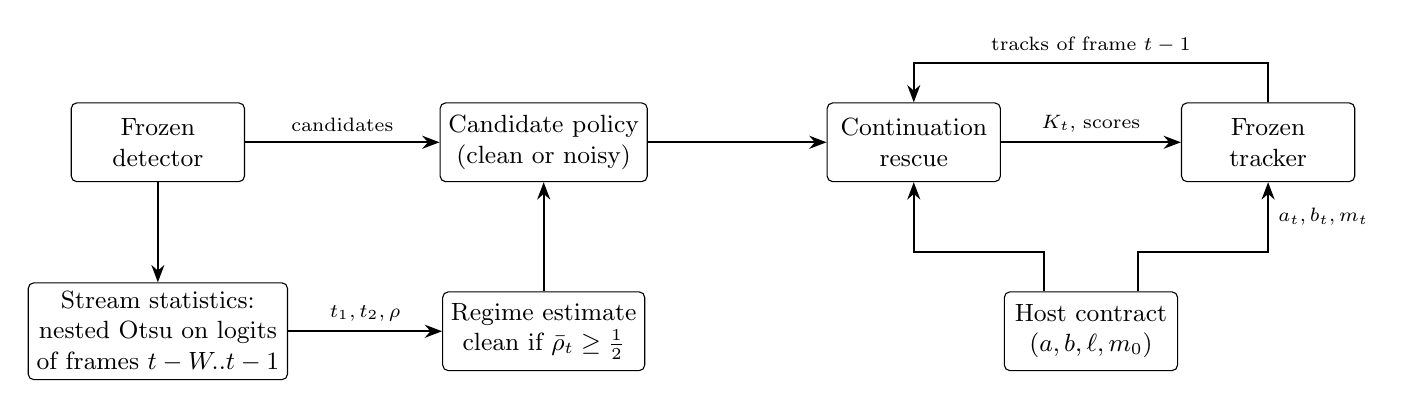
\begin{tikzpicture}[
  box/.style={draw, rounded corners=2pt, align=center, font=\small, minimum height=10mm, minimum width=22mm, inner sep=3pt},
  arr/.style={-{Stealth[length=2.2mm]}, thick}, lab/.style={font=\scriptsize}]
\node[box] (det) at (0,0) {Frozen\\detector};
\node[box] (pol) at (4.9,0) {Candidate policy\\(clean or noisy)};
\node[box] (res) at (9.6,0) {Continuation\\rescue};
\node[box] (trk) at (14.1,0) {Frozen\\tracker};
\node[box] (stat) at (0,-2.4) {Stream statistics:\\nested Otsu on logits\\of frames $t-W..t-1$};
\node[box] (reg) at (4.9,-2.4) {Regime estimate\\clean if $\bar\rho_t \ge \tfrac12$};
\node[box] (hc) at (11.85,-2.4) {Host contract\\$(a, b, \ell, m_0)$};
\draw[arr] (det) -- node[lab, above]{candidates} (pol);
\draw[arr] (pol) -- (res);
\draw[arr] (res) -- node[lab, above]{$K_t$, scores} (trk);
\draw[arr] (det) -- (stat);
\draw[arr] (stat) -- node[lab, above]{$t_1, t_2, \rho$} (reg);
\draw[arr] (reg) -- (pol);
\draw[arr] (hc.north) ++(-0.6,0) |- ++(0,0.5) -| (res.south);
\draw[arr] (hc.north) ++(0.6,0) |- ++(0,0.5) -| node[lab, pos=0.75, right]{$a_t, b_t, m_t$} (trk.south);
\draw[arr] (trk.north) -- ++(0,0.5) -| node[lab, pos=0.25, above]{tracks of frame $t-1$} (res.north);
\end{tikzpicture}}
\caption{Self-calibrating control layer between a frozen detector and a frozen tracker. Statistics use earlier frames only; the host contract is the tracker's published operating point; the tracker receives the selected candidates, their scores, and its thresholds for the frame.}
\label{fig:ch5-arch}
\end{figure}

\section{Causal Self-Calibration}\label{sec:ch5-calib}
The layer pools the logits of all candidates of the previous $W=10$ frames and splits them twice with the exact Otsu threshold \cite{otsu1979}: the first split $t_1$ separates background from foreground, and a second split of the foreground, $t_2$, separates ambiguous from confident candidates. The confident share of the foreground,
\begin{equation}
\rho_t = \frac{\left|\{i: z_i \ge t_2\}\right|}{\left|\{i: z_i \ge t_1\}\right|},
\label{eq:ch5-rho}
\end{equation}
summarizes how cleanly the detector separates objects from clutter. Working on logits makes the splits invariant to affine transforms of the logit, such as a change of temperature; the host's thresholds are compared on the same scale.

The bands are interpretable only if the stream has a background mode. When the class below $t_1$ holds fewer pooled candidates than the foreground, which happens when a detector emits few low-scoring candidates, the first split falls inside the objects and $\rho$ would falsely signal clutter. In that case the frame counts as clean evidence ($\rho_t=1$). This interpretability check was added after a development diagnosis in which sequence starts with about ten candidates per frame produced splits at $t_1\approx0.6$ and $t_2\approx0.93$ in probability terms and a false noisy call.

\section{Intervention Regimes}\label{sec:ch5-regimes}

\subsection{Regime estimate}
The stream is clean at frame $t$ if the median $\bar\rho_t$ of $\rho$ over all past non-cold frames is at least one half; otherwise it is noisy. The regime is thus a property of the detector and scene stream rather than of a single frame, so that a transient confidence dip, for example under fast camera motion, does not flip it. Before the first valid split (the first frame of a stream), the regime is cold.

\subsection{Cold and clean regimes: self-limiting}
In the cold and clean regimes the tracker's own thresholds are kept, and they are lowered only as far as $t_2$ when the tracker would otherwise reject the confident class: $a_t=\min(a, \sigma(t_2))$ and likewise for $b_t$, where $\sigma$ is the logistic function. Scores are passed unchanged, and only cross-class duplicates, that is, one box proposed with two class labels, are removed. On a stream whose confident class lies above the tracker's thresholds, the tracker therefore receives exactly its native input.

\subsection{Noisy regime: banded intervention}
In the noisy regime the candidates are banded: the primary band $z\ge t_2$ may start and continue tracks, the extension band $t_1\le z<t_2$ may continue tracks but not start them, and candidates below $t_1$ are discarded. Scores are remapped through their empirical distribution in the stream, primary candidates to $[0.5,1)$ and extension candidates to $[0.1,0.5)$, and the tracker's association and birth thresholds are set to 0.5, so that extension candidates can reach only a tracker's low stage. Duplicates are resolved with track context: a weaker candidate overlapping a stronger one (overlap above one half) is removed unless a different track of the previous frame claims it, which keeps occluded people in crowds.

\subsection{Continuation rescue}
A foreground candidate ($z\ge t_1$; every emitted candidate when the stream has no background mode) that continues an existing track of frame $t-1$ with overlap at least one half, where no usable candidate covers that track and the tracker could not see the candidate at the operating point passed this frame, is passed to the tracker with its score raised just above the lowest threshold the tracker uses at that frame. For a two-stage tracker this band is empty by construction because $\ell$ already admits such candidates; for a single-stage tracker it supplies the continuation stage the tracker lacks.

\subsection{Motion rule}
In noisy frames only, and only when an image-motion cue is available, the matching tolerance widens with the ratio $r_t$ of the current global image motion (phase correlation on a quarter-resolution frame \cite{reddy1996phasecorr}) to its past median:
\begin{equation}
m_t=\min\left(0.95,\; 1-\frac{1-m_0}{\max(1,r_t)}\right).
\label{eq:ch5-motion}
\end{equation}


\subsection{Per-frame decision}
Algorithm~\ref{alg:ch5-layer} summarizes the decision of the layer for one frame. Every statistic that decides the regime and the thresholds is computed from earlier frames; the logits of frame $t$ enter the buffer only after the decision.

\begin{algorithm}[tbp]
\caption{Per-frame decision of the self-calibrating control layer (frozen configuration).}
\label{alg:ch5-layer}
\small
\begin{algorithmic}[1]
\Require candidates $\{(\mathbf{x}_i,s_i,c_i)\}$ of frame $t$; logit buffer $H$ of frames $t-W,\ldots,t-1$; history $R$ of $\rho$; tracks $\mathcal{T}_{t-1}$; host contract $(a,b,\ell,m_0)$; optional motion ratio $r_t$
\Ensure passed candidates $K_t$, their scores, thresholds $a_t, b_t$, tolerance $m_t$
\If{$H$ admits no valid split}
  \State regime $\gets$ cold;\quad $(a_t,b_t)\gets(a,b)$
\Else
  \State $t_1 \gets \mathrm{Otsu}(H)$;\quad $t_2 \gets \mathrm{Otsu}(\{z\in H: z\ge t_1\})$
  \State $\rho_t \gets |\{z\in H: z\ge t_2\}| \,/\, |\{z\in H: z\ge t_1\}|$
  \If{$|\{z\in H: z<t_1\}| < |\{z\in H: z\ge t_1\}|$} \Comment{no background mode}
    \State $\rho_t \gets 1$
  \EndIf
  \State append $\rho_t$ to $R$;\quad $\bar\rho_t \gets \mathrm{median}(R)$
  \If{$\bar\rho_t \ge 1/2$}
    \State regime $\gets$ clean;\quad $a_t \gets \min(a,\sigma(t_2))$;\quad $b_t \gets \min(b,\sigma(t_2))$
  \Else
    \State regime $\gets$ noisy;\quad discard candidates with $z_i<t_1$
    \State remap scores by their stream ECDF: $z_i\ge t_2 \mapsto [0.5,1)$, $t_1\le z_i<t_2 \mapsto [0.1,0.5)$
    \State $a_t \gets 0.5$;\quad $b_t \gets 0.5$
  \EndIf
\EndIf
\If{regime is noisy}
  \State remove weaker overlapping candidates (IoU $>0.5$) unless a different track of $\mathcal{T}_{t-1}$ claims them
\Else
  \State remove cross-class duplicates only; pass scores unchanged
\EndIf
\ForAll{tracks $\tau\in\mathcal{T}_{t-1}$ not covered by a usable candidate}
  \State pass the strongest foreground candidate with IoU $\ge 0.5$ to $\tau$ that the tracker cannot see this frame, with its score raised just above the lowest threshold the tracker uses
\EndFor
\State $m_t \gets m_0$;\quad \textbf{if} regime is noisy and $r_t$ is available \textbf{then} $m_t \gets \min\!\left(0.95,\,1-(1-m_0)/\max(1,r_t)\right)$
\State append the logits of frame $t$ to $H$ and drop frames older than $t-W+1$
\end{algorithmic}
\end{algorithm}

\section{Host Contract and Adapters}\label{sec:ch5-contract}
Table~\ref{tab:ch5-contracts} lists the contracts used. Each value is a documented property of the published tracker configuration, not a fitted quantity. An adapter per tracker family maps the layer's decision onto the tracker's interface: the selected candidates and their scores replace the detector output of the frame, and the thresholds and tolerance replace the tracker's own for that frame. Where a tracker has no overlap gate (C-TWiX) or two detection views (TrackTrack), the adapter maps only what the tracker exposes; in TrackTrack's second view a detection that matches a candidate at overlap 0.97 or more, the tracker's own rule, follows that candidate. Post-processing that the authors apply after tracking (interpolation, offline linking) is kept unchanged and evaluated as in the original papers. Tracker-agnostic is meant in this sense: the policy and all of its parameters are identical for every tracker, a tracker enters only through its published contract values, and the adapter translates the decision without making one.

\begin{table}[tbp]
\centering
\caption{Host contracts: the operating point each published tracker declares, as used by the layer. $\tau$ is the tracker's own published threshold, which differs between trackers and, for TrackTrack, between sequences.}
\label{tab:ch5-contracts}
\small\setlength{\tabcolsep}{4pt}
\begin{adjustbox}{max width=\textwidth}
\begin{tabular}{>{\raggedright\arraybackslash}p{3.4cm}ccccc>{\raggedright\arraybackslash}p{3.6cm}}
\hline
Tracker (setting) & Type & assoc & birth & low & match & Decision mapped to \\
\hline
ByteTrack (official MOT17) & two-stage & 0.6 & 0.7 & 0.1 & 0.8 & thresholds, candidates, scores \\
ByteTrack (library default) & two-stage & 0.25 & 0.25 & 0.1 & 0.8 & same \\
SparseTrack & two-stage & $\tau$ & $\tau+0.1$ & 0.1 & published & same \\
BoostTrack & two-stage & $\tau$ & $\tau$ & 0.1 & $1-$IoU gate & same \\
Hybrid-SORT & two-stage & $\tau$ & $\tau$ & 0.1 & $1-$IoU gate & same \\
OC-SORT & single-stage & 0.6 & 0.6 & 0.6 & 0.7 & same \\
PD-SORT & single-stage & $\tau$ & $\tau$ & $\tau$ & $1-$IoU gate & same \\
C-TWiX (MOT17 / KITTI / DanceTrack) & single-stage & 0.5 & 0.7 / 0.5 / 0.9 & 0.5 & not mapped & candidates, scores, two score thresholds \\
TrackTrack & two-view & $\tau_{\mathrm{det}}$ & $\tau_{\mathrm{init}}$ & 0.1 & not mapped & candidates in both views, two thresholds \\
\hline
\end{tabular}
\end{adjustbox}
\end{table}


\section{Complexity}\label{sec:ch5-complexity}
Per frame the layer sorts the pooled logits of at most $W$ frames for the two Otsu splits, computes candidate overlaps with the candidates and with the previous frame's tracks, and, when the motion cue is used, computes one phase correlation on a quarter-resolution image. With $n$ candidates per frame and $k$ tracks, the cost is $O(Wn\log(Wn) + n^2 + nk)$ plus the fixed image cost. The state is a ring buffer of $W$ frames of logits and a history of 100 motion ratios.

\section{Development and Freeze Protocol}\label{sec:ch5-protocol}

\subsection{Design history}
The layer evolved from an earlier design of the same research program that always intervened: it banded the stream with the same thresholds, removed every overlapping duplicate, and remapped scores in every frame. That design helped with miscalibrated and noisy detectors but hurt strong published trackers: on MOT17 it cost SparseTrack 4.15 HOTA points ($[-5.54,-1.66]$) and BoostTrack 5.89 points ($[-7.76,-2.87]$), because overlap-based duplicate removal deleted occluded people in crowds and its self-calibrated thresholds were stricter than the trackers' own (false positives fell by 1,630 and 1,351, false negatives rose by 4,955 and 6,167). Figure~\ref{fig:ch5-v6} shows that failure and the result of the frozen layer on the same trackers. The regime estimate, the self-limiting clean regime, track-context duplicates, the whole-stream regime, the interpretability check, and the continuation rescue were each introduced to remove a diagnosed failure (Table~\ref{tab:ch5-ablation}).

\begin{figure}[tbp]
\centering
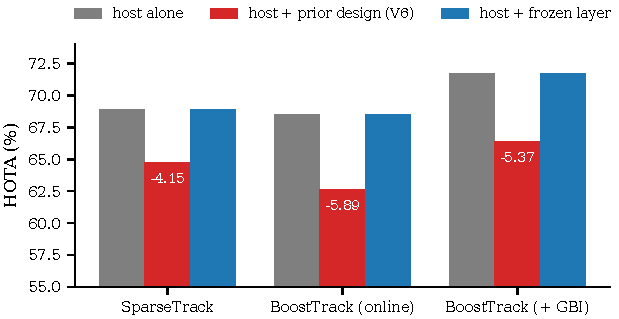
\includegraphics[width=0.7\textwidth]{figures/ch5_fig2_v6_to_v7.pdf}
\caption{The design problem: the prior always-intervening design degraded strong published trackers on MOT17 (difference in white); the frozen layer leaves them at their own accuracy.}
\label{fig:ch5-v6}
\end{figure}

\begin{table}[tbp]
\centering
\caption{Design steps from the prior always-intervening design to the frozen policy (development data, HOTA \%), and variants tested and rejected.}
\label{tab:ch5-ablation}
\small\setlength{\tabcolsep}{4pt}
\begin{adjustbox}{max width=\textwidth}
\begin{tabular}{>{\raggedright\arraybackslash}p{3.1cm}>{\raggedright\arraybackslash}p{4.8cm}>{\raggedright\arraybackslash}p{6.9cm}}
\hline
Step & Change & Effect \\
\hline
V6 emulated inside V7 & always-noisy bands, overlap deduplication, rank remap & ByteTrack (0.1) 56.41 vs host 67.70; OC-SORT (0.1) 45.72 vs 66.44 \\
V7a--V7d & regime statistic, host-anchored clean regime, crowd-safe duplicates & SparseTrack 64.72 to 68.93 (host 68.88); BoostTrack 62.61 to 68.37 (host 68.49) \\
+ whole-stream regime & regime from all past frames & ByteTrack (0.1) 67.561 to 67.702; OC-SORT (0.1) 65.697 to 66.071 \\
+ continuation rescue & foreground track-consistent rescue & OC-SORT (0.01) 66.405 to 66.619; OC-SORT (0.1) 66.071 to 66.469 \\
+ interpretability check = V7f & no background mode gives no evidence against the host & ByteTrack/BoostTrack (0.1) identical to host; OC-SORT 67.041 (0.01), 66.907 (0.1) \\
\hline
\multicolumn{2}{l}{\textit{Rejected variant}} & \textit{Evidence} \\
\multicolumn{2}{>{\raggedright\arraybackslash}p{8.0cm}}{no candidates at frame 1} & -0.3 to -0.5 HOTA on every MOT17 host \\
\multicolumn{2}{>{\raggedright\arraybackslash}p{8.0cm}}{rescue below a two-stage host's low stage} & FP +700 to +1000, -0.4 to -0.5 HOTA \\
\multicolumn{2}{>{\raggedright\arraybackslash}p{8.0cm}}{rank-remapped scores in clean frames} & ByteTrack -0.2 / -1.6 HOTA \\
\multicolumn{2}{>{\raggedright\arraybackslash}p{8.0cm}}{host-clipped noisy primary band} & KITTI YOLOv8n ByteTrack +1.4 HOTA but uncontrolled false tracks on a noisy aerial stream (26.9 vs 14.9 boxes/frame) \\
\hline
\end{tabular}
\end{adjustbox}
\end{table}


\subsection{Freeze and evaluation roles}
The final configuration was frozen before any external evaluation, recorded in a version-control tag, and protected by a lock file of cryptographic hashes of the layer, its configuration, and the evaluation runners; every post-freeze run verified the lock before running. Sixty-one automated tests check causality, state reset, pass-through on clean streams, independence from names, invariance to affine score transforms where designed, and lock integrity. Table~\ref{tab:ch5-data} lists the evaluation cells and their roles. Development cells (MOT17 with four trackers, KITTI with three trackers and two detectors, score-transform stress tests) were visible during design, so their gains are measured but not held out. The predeclared external systems (PD-SORT, Hybrid-SORT) were selected and declared before they were run, and run once. The post-freeze external systems (C-TWiX, TrackTrack, TOPICTrack) were selected under a protocol registered before any run, which fixed the host contracts, the reproduction criteria, and predictions of the layer's effect; a system entered the analysis only if its baseline reproduced the authors' number (EXACT: within 0.2 HOTA; CLOSE: within 1.0 with a documented, untuned cause).

\begin{table}[tbp]
\centering
\caption{Evaluation cells and their role. Development cells were visible while the layer was designed; predeclared and post-freeze cells were run once with the frozen policy.}
\label{tab:ch5-data}
\small\setlength{\tabcolsep}{4pt}
\begin{adjustbox}{max width=\textwidth}
\begin{tabular}{>{\raggedright\arraybackslash}p{3.0cm}>{\raggedright\arraybackslash}p{3.6cm}>{\raggedright\arraybackslash}p{4.6cm}>{\raggedright\arraybackslash}p{3.2cm}}
\hline
Data & Detector & Trackers & Role \\
\hline
MOT17 val-half (7 sequences) & published YOLOX-X detections & ByteTrack (2 settings), OC-SORT, BoostTrack, SparseTrack & development \\
KITTI tracking training (21 sequences) & YOLOv8n, RT-DETR-L & ByteTrack, BoT-SORT, OC-SORT & development (detector transfer) \\
MOT17 val-half, score transforms & published YOLOX-X, transformed scores & ByteTrack (2 settings), OC-SORT, BoostTrack & development (robustness) \\
MOT17 val-half & released PD-SORT / Hybrid-SORT detections & PD-SORT, Hybrid-SORT & predeclared external \\
MOT17 val-half, KITTI MOTS val (9 sequences), DanceTrack val (25 sequences) & authors' released detections & C-TWiX, TrackTrack (DanceTrack), TOPICTrack (MOT17) & post-freeze external \\
\hline
\end{tabular}
\end{adjustbox}
\end{table}


\subsection{Statistics}
All comparisons are paired: both arms use the same detections and the same environment. Differences are pooled over sequences and their 95\% intervals come from a percentile bootstrap over sequences with 10,000 resamples and seed 42 \cite{efron1993bootstrap}. A difference is called significant only when its interval excludes zero. Per-sequence wins, ties ($|\Delta\mathrm{HOTA}|<0.01$), and losses are reported as a distribution-free complement. Evaluation uses TrackEval (commit 12c8791) with the official ground truth of each benchmark.

\section{Tracker Transfer}\label{sec:ch5-tracker}
Table~\ref{tab:ch5-mot17} gives the development trackers on MOT17 val-half with the published YOLOX-X detections, and Fig.~\ref{fig:ch5-forest} summarizes every cell of the chapter.

\begin{sidewaystable}
\centering
\caption{Development hosts on MOT17 val-half (published YOLOX-X detections). Host = our reproduction; $\Delta$ = host with the frozen layer minus host, with 95\% paired-bootstrap interval (10,000 resamples, seed 42); bold intervals exclude zero. The floor is the lowest detector score emitted.}
\label{tab:ch5-mot17}
\small\setlength{\tabcolsep}{4pt}
\begin{adjustbox}{max width=\textheight}
\begin{tabular}{llllccc}
\hline
Tracker & Setting & Paper HOTA / MOTA / IDF1 & Host HOTA / MOTA / IDF1 & $\Delta$HOTA & $\Delta$MOTA & $\Delta$IDF1 \\
\hline
SparseTrack & -- & 69.2 / 76.8 / 81.4 & 68.88 / 77.85 / 81.97 & $+0.06$ [$-0.01$, $+0.25$] & $+0.08$ [$-0.03$, $+0.30$] & $+0.16$ [$-0.01$, $+0.70$] \\
BoostTrack & online & 68.37 / 75.56 / 81.35 & 68.49 / 75.50 / 81.41 & 0 (identical) & 0 (identical) & 0 (identical) \\
BoostTrack & + GBI & 71.33 / 80.55 / 83.84 & 71.72 / 81.03 / 84.16 & 0 (identical) & 0 (identical) & 0 (identical) \\
ByteTrack & floor 0.01 & -- / 76.6 / 79.3 & 67.70 / 77.60 / 79.47 & $-0.014$ [$-0.058$, $+0.009$] & $+0.06$ [$-0.15$, $+0.34$] & $-0.03$ [$-0.14$, $+0.04$] \\
ByteTrack & floor 0.1 & -- / 76.6 / 79.3 & 67.70 / 77.60 / 79.47 & 0 (identical) & 0 (identical) & 0 (identical) \\
OC-SORT & floor 0.01 & 66.5 / 74.9 / 77.7 & 66.43 / 74.67 / 78.05 & {\boldmath $+0.61$ [$+0.36$, $+1.24$]} & {\boldmath $+1.27$ [$+0.17$, $+3.01$]} & $+0.66$ [$-0.25$, $+1.60$] \\
OC-SORT & floor 0.1 & 66.5 / 74.9 / 77.7 & 66.44 / 74.67 / 78.05 & {\boldmath $+0.46$ [$+0.27$, $+1.09$]} & {\boldmath $+1.26$ [$+0.37$, $+3.34$]} & {\boldmath $+0.287$ [$+0.003$, $+0.838$]} \\
\hline
\end{tabular}
\end{adjustbox}
\end{sidewaystable}


\begin{figure}[tbp]
\centering
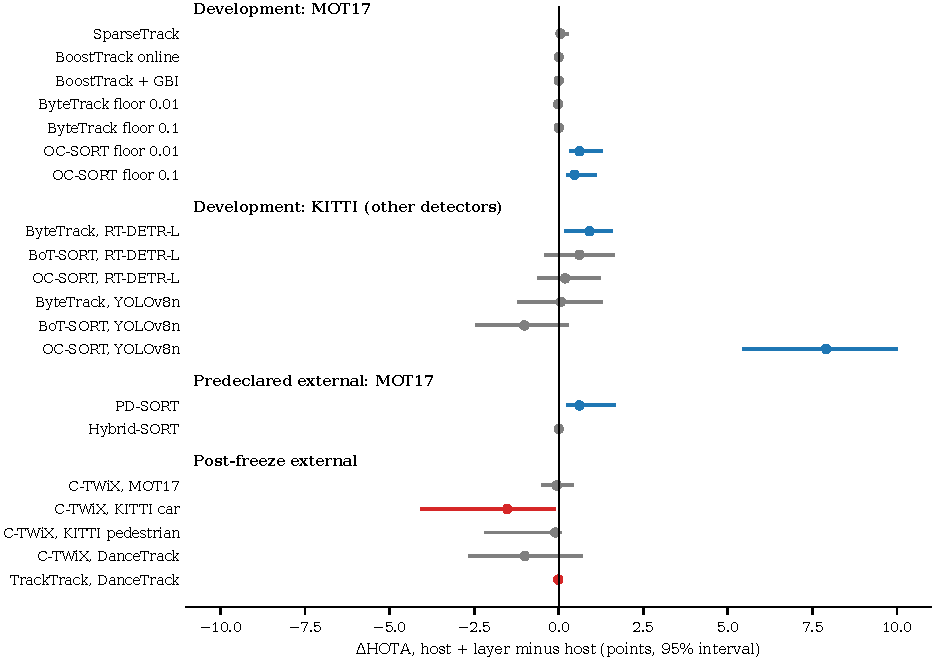
\includegraphics[width=0.92\textwidth]{figures/ch5_fig3_forest.pdf}
\caption{Every evaluated cell: difference in HOTA (tracker with the frozen layer minus tracker alone) with 95\% paired-bootstrap interval. Blue: interval above zero; red: below zero; gray: includes zero or identical output.}
\label{fig:ch5-forest}
\end{figure}

The two-stage trackers with well-matched detections were left unchanged. BoostTrack (online and with interpolation) and ByteTrack at floor 0.1 produced identical output; ByteTrack at floor 0.01 changed by $-0.014$ ($[-0.058,+0.009]$); SparseTrack changed by $+0.055$ ($[-0.011,+0.254]$). This is the intended self-limiting behavior, and it is the result the prior design could not achieve (Fig.~\ref{fig:ch5-v6}).

The single-stage OC-SORT improved at both emission floors: HOTA $+0.61$ ($[+0.36,+1.24]$) and $+0.46$ ($[+0.27,+1.09]$), MOTA $+1.27$ and $+1.26$, with gains on 7 of 7 sequences in both settings (Fig.~\ref{fig:ch5-perseq}). The mechanism is the continuation rescue: OC-SORT discards every detection below its single threshold, and the layer hands it the foreground candidates that continue an unmatched track.

\begin{figure}[tbp]
\centering
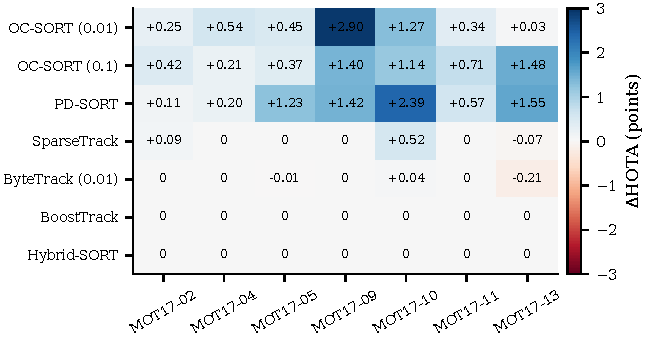
\includegraphics[width=0.7\textwidth]{figures/ch5_fig4_per_sequence.pdf}
\caption{Per-sequence HOTA differences on MOT17 val-half for development and predeclared trackers.}
\label{fig:ch5-perseq}
\end{figure}

\section{Detector Transfer}\label{sec:ch5-detector}

\subsection{A different detector and dataset}
On KITTI tracking training, three trackers were run with two detectors other than the MOT17 detector (Table~\ref{tab:ch5-kitti}). With the noisy RT-DETR-L stream \cite{zhao2024rtdetr}, the two-stage trackers gained substantially in MOTA and IDF1: ByteTrack $+5.98$ MOTA ($[+1.16,+9.94]$) and $+3.87$ IDF1, BoT-SORT $+7.86$ MOTA ($[+2.21,+13.44]$) and $+3.10$ IDF1, with HOTA $+0.91$ ($[+0.22,+1.55]$) for ByteTrack. With YOLOv8n, the single-stage OC-SORT gained 7.91 HOTA ($[+5.47,+9.98]$), while ByteTrack and BoT-SORT lost MOTA ($-1.87$ and $-2.43$, the latter significant) while their identity switches fell by about half; this regression is analyzed in Sec.~\ref{sec:ch5-failures}.

\begin{sidewaystable}
\centering
\caption{Detector transfer on KITTI tracking training (official HOTA, car and pedestrian averaged). BoT-SORT excludes one sequence on which the unmodified tracker fails numerically.}
\label{tab:ch5-kitti}
\small\setlength{\tabcolsep}{4pt}
\begin{adjustbox}{max width=\textheight}
\begin{tabular}{llcccc}
\hline
Tracker & Detector & Host HOTA / MOTA / IDF1 & $\Delta$HOTA & $\Delta$MOTA & $\Delta$IDF1 \\
\hline
ByteTrack & RT-DETR-L & 50.73 / 47.27 / 64.98 & {\boldmath $+0.91$ [$+0.22$, $+1.55$]} & {\boldmath $+5.98$ [$+1.16$, $+9.94$]} & {\boldmath $+3.87$ [$+1.67$, $+5.06$]} \\
BoT-SORT & RT-DETR-L & 53.91 / 48.25 / 67.74 & $+0.61$ [$-0.39$, $+1.61$] & {\boldmath $+7.86$ [$+2.21$, $+13.44$]} & {\boldmath $+3.10$ [$+1.00$, $+4.57$]} \\
OC-SORT & RT-DETR-L & 52.64 / 57.59 / 69.87 & $+0.19$ [$-0.57$, $+1.19$] & $-0.57$ [$-4.36$, $+1.40$] & $+0.04$ [$-1.31$, $+1.78$] \\
ByteTrack & YOLOv8n & 45.31 / 46.54 / 60.92 & $+0.06$ [$-1.19$, $+1.24$] & $-1.87$ [$-6.25$, $+0.03$] & $+1.49$ [$-0.36$, $+3.27$] \\
BoT-SORT & YOLOv8n & 49.21 / 49.89 / 64.41 & $-1.02$ [$-2.43$, $+0.25$] & {\boldmath $-2.43$ [$-7.43$, $-0.14$]} & $+0.35$ [$-2.10$, $+2.27$] \\
OC-SORT & YOLOv8n & 36.27 / 33.99 / 50.46 & {\boldmath $+7.91$ [$+5.47$, $+9.98$]} & {\boldmath $+9.40$ [$+1.10$, $+12.30$]} & {\boldmath $+9.60$ [$+5.61$, $+12.16$]} \\
\hline
\end{tabular}
\end{adjustbox}
\end{sidewaystable}


\subsection{Detector confidence shift}
To isolate the calibration problem, the published MOT17 detections were transformed before the tracker by four monotone maps: cubing ($s^3$), halving ($0.5s$), and logit temperatures 2 and 0.5 (Fig.~\ref{fig:ch5-shift}). The trackers kept their published thresholds. Halving the scores drove ByteTrack (official setting) and OC-SORT to 0 HOTA because no detection reached their thresholds; with the layer they reached 66.17 and 66.72. Cubing reduced them to 60.92 and 58.34; with the layer they reached 65.81 and 66.60, and BoostTrack went from 61.33 to 64.84. Under the temperatures the layer gained up to 1.23 points or left the output unchanged. The ByteTrack library setting, whose low thresholds already admit the shifted scores, was unchanged within 0.14 points in all four transforms. These cells are development evidence. Their paired intervals were computed after the freeze on the recorded runs, whose replay reproduced every recorded metric exactly (Table~\ref{tab:ch5-shiftboot}): the layer recovered significantly in 7 of the 14 conditions and degraded significantly in none, and the other 7 were identical or had intervals including zero.

\begin{table}[tbp]
\centering
\caption{Detector confidence shift on MOT17 val-half with 95\% paired-bootstrap intervals (10,000 resamples, seed 42), computed after the freeze on the recorded runs. HOTA of each tracker with its published thresholds, alone and with the frozen layer; bold intervals exclude zero; W/T/L are per-sequence wins, ties, and losses.}
\label{tab:ch5-shiftboot}
\small\setlength{\tabcolsep}{4pt}
\begin{adjustbox}{max width=\textwidth}
\begin{tabular}{llrrlc}
\hline
Tracker (setting) & Transform & Alone & With layer & $\Delta$HOTA & W/T/L \\
\hline
ByteTrack (official setting) & $s^3$ & 60.92 & 65.81 & {\boldmath $+4.89$ [$+2.60$, $+13.69$]} & 7/0/0 \\
ByteTrack (official setting) & $0.5s$ & 0.00 & 66.17 & {\boldmath $+66.17$ [$+49.32$, $+75.40$]} & 7/0/0 \\
ByteTrack (official setting) & temperature 2 & 65.84 & 66.95 & {\boldmath $+1.11$ [$+0.35$, $+3.87$]} & 6/0/1 \\
ByteTrack (official setting) & temperature 0.5 & 67.30 & 67.29 & $-0.01$ [$-0.05$, $+0.00$] & 1/4/2 \\
ByteTrack (library setting) & $s^3$ & 66.31 & 66.31 & $-0.01$ [$-0.38$, $+0.38$] & 3/0/4 \\
ByteTrack (library setting) & $0.5s$ & 66.61 & 66.48 & $-0.14$ [$-0.66$, $+0.14$] & 2/3/2 \\
ByteTrack (library setting) & temperature 2 & 63.97 & 63.97 & 0 (identical) & 0/7/0 \\
ByteTrack (library setting) & temperature 0.5 & 66.53 & 66.52 & $-0.01$ [$-0.03$, $+0.00$] & 0/5/2 \\
OC-SORT & $s^3$ & 58.34 & 66.60 & {\boldmath $+8.26$ [$+5.86$, $+16.81$]} & 7/0/0 \\
OC-SORT & $0.5s$ & 0.00 & 66.72 & {\boldmath $+66.72$ [$+50.32$, $+75.56$]} & 7/0/0 \\
OC-SORT & temperature 2 & 65.99 & 67.22 & {\boldmath $+1.24$ [$+0.52$, $+3.42$]} & 6/0/1 \\
OC-SORT & temperature 0.5 & 66.61 & 67.06 & $+0.45$ [$-0.01$, $+0.97$] & 4/0/3 \\
BoostTrack online & $s^3$ & 61.33 & 64.84 & {\boldmath $+3.51$ [$+0.85$, $+13.28$]} & 7/0/0 \\
BoostTrack online & temperature 2 & 67.59 & 67.59 & 0 (identical) & 0/7/0 \\
\hline
\end{tabular}
\end{adjustbox}
\end{table}


\begin{figure}[tbp]
\centering
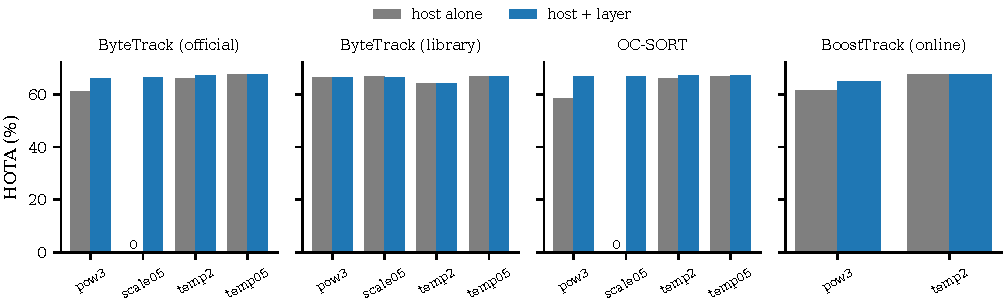
\includegraphics[width=\textwidth]{figures/ch5_fig5_calibration_shift.pdf}
\caption{Detector confidence shift on MOT17 val-half: HOTA of each published tracker with its published thresholds, alone and with the frozen layer, after four monotone transforms of the detector scores.}
\label{fig:ch5-shift}
\end{figure}

\section{Post-Freeze External Evaluation}\label{sec:ch5-external}
Table~\ref{tab:ch5-external} gives every external system evaluated with the frozen layer.

\begin{sidewaystable}
\centering
\caption{External systems evaluated once with the frozen layer. Reproduction class against the authors' reported number (EXACT: $|\Delta\mathrm{HOTA}|\le0.2$; CLOSE: $\le1.0$ with a documented, untuned cause). TOPICTrack failed reproduction and is excluded from the analysis.}
\label{tab:ch5-external}
\small\setlength{\tabcolsep}{4pt}
\begin{adjustbox}{max width=\textheight}
\begin{tabular}{llllccc}
\hline
System & Data & Reference / reproduced HOTA & Class & $\Delta$HOTA & $\Delta$MOTA & $\Delta$IDF1 \\
\hline
\multicolumn{7}{l}{\textit{Predeclared before the runs}}\\
PD-SORT & MOT17 val-half & 68.01 / 68.01 & EXACT (released output) & {\boldmath $+0.61$ [$+0.27$, $+1.65$]} & {\boldmath $+1.13$ [$+0.27$, $+3.03$]} & {\boldmath $+0.82$ [$+0.43$, $+1.94$]} \\
Hybrid-SORT & MOT17 val-half & 67.1 / 66.70 & CLOSE & 0 (identical) & 0 (identical) & 0 (identical) \\
\multicolumn{7}{l}{\textit{Post-freeze, protocol registered before the runs}}\\
C-TWiX & MOT17 val-half & 77.8 / 77.55 & CLOSE & $-0.05$ [$-0.46$, $+0.40$] & $+0.24$ [$-0.58$, $+1.12$] & $+0.18$ [$-0.47$, $+1.14$] \\
C-TWiX (car) & KITTI MOTS val & 89.3 / 89.27 & EXACT & {\boldmath $-1.52$ [$-4.05$, $-0.13$]} & {\boldmath $-2.11$ [$-5.89$, $-0.17$]} & {\boldmath $-1.21$ [$-3.32$, $-0.10$]} \\
C-TWiX (pedestrian) & KITTI MOTS val & 71.4 / 70.77 & CLOSE & $-0.10$ [$-2.16$, $+0.03$] & $-0.31$ [$-4.86$, $+0.10$] & $-0.01$ [$-1.90$, $+0.08$] \\
C-TWiX & DanceTrack val & 60.4 / 59.62 & CLOSE & $-1.00$ [$-2.62$, $+0.65$] & $+0.13$ [$-0.39$, $+0.47$] & $-1.55$ [$-3.76$, $+0.52$] \\
TOPICTrack & MOT17 val-half & 69.6 / 67.54 & FAILED & \multicolumn{3}{c}{not analyzed} \\
TrackTrack & DanceTrack val & 63.3 / 62.96 & CLOSE & {\boldmath $-0.013$ [$-0.032$, $-0.001$]} & {\boldmath $-0.073$ [$-0.208$, $-0.004$]} & $+0.009$ [$-0.001$, $+0.028$] \\
\hline
\end{tabular}
\end{adjustbox}
\end{sidewaystable}


\subsection{Predeclared systems}
PD-SORT \cite{wang2025pdsort} was reproduced identically to the authors' released output. With the layer, HOTA rose by 0.61 ($[+0.27,+1.65]$), MOTA by 1.13 ($[+0.27,+3.03]$), and IDF1 by 0.82 ($[+0.43,+1.94]$), with HOTA higher on 7 of 7 sequences (Fig.~\ref{fig:ch5-perseq}). False negatives fell by 1,291 and false positives rose by 681. PD-SORT is single-stage, and the gain follows the same mechanism as for OC-SORT; unlike OC-SORT, PD-SORT was not seen during design. Hybrid-SORT \cite{yang2024hybridsort}, a two-stage tracker, produced identical output, as predicted.

\subsection{Recent systems after the freeze}
C-TWiX \cite{miah2025twix} was reproduced on three datasets (Table~\ref{tab:ch5-external}). On MOT17 the layer changed HOTA by $-0.05$ ($[-0.46,+0.40]$) with MOTA $+0.24$ and IDF1 $+0.18$; on KITTI pedestrians by $-0.10$ ($[-2.16,+0.03]$); on DanceTrack by $-1.00$ ($[-2.62,+0.65]$) with an IDF1 loss of 1.55 whose interval includes zero. On KITTI cars it lost 1.52 HOTA ($[-4.05,-0.13]$), the one significant external degradation of the paper (Sec.~\ref{sec:ch5-failures}). TrackTrack \cite{shim2025tracktrack} was reproduced within 0.34 HOTA on DanceTrack; the layer changed its HOTA by $-0.013$ ($[-0.032,-0.001]$), a significant but negligible difference, with 21 of 25 sequences tied. TOPICTrack \cite{cao2025topictrack} failed the registered reproduction criterion (67.54 against 69.6 HOTA) and is excluded; the frozen layer's effect on it ($-0.016$, interval including zero) is recorded but not analyzed.

\section{Cross-Dataset Analysis}\label{sec:ch5-cross}
Across MOT17, KITTI, and DanceTrack, the direction of the effect is predicted by two properties of the pipeline rather than by the dataset: whether the tracker has a continuation stage and whether the detector's score distribution matches the tracker's thresholds. The regime estimate makes this visible (Fig.~\ref{fig:ch5-regimes}a): on the post-freeze streams, 99.7\% of MOT17 frames and 99.9\% of DanceTrack frames were classified clean, and the layer left those pipelines at or near their native output. KITTI had the largest noisy share (2.8\% of frames), concentrated in short sequences.

\begin{figure}[tbp]
\centering
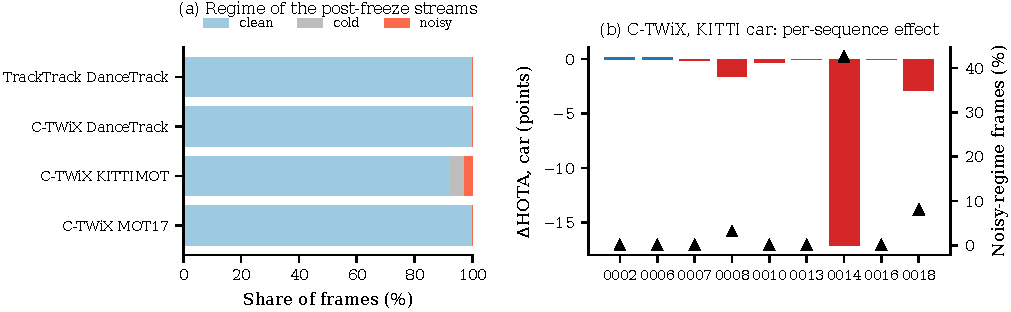
\includegraphics[width=\textwidth]{figures/ch5_fig6_regimes_failure.pdf}
\caption{(a) Share of frames in each regime on the post-freeze streams. (b) C-TWiX on KITTI cars: per-sequence HOTA difference (bars) and share of frames classified noisy (triangles); the loss concentrates in sequence 0014.}
\label{fig:ch5-regimes}
\end{figure}

\section{Robustness Analysis}\label{sec:ch5-robust}
Three kinds of robustness were measured. Score transforms (Sec.~\ref{sec:ch5-detector}) test calibration shift with the detections fixed; the worst cell was $-0.14$ HOTA, with an interval including zero. Emission floors test how much of the low-score tail the detector emits: on MOT17 the two-stage trackers were unchanged at floors 0.01 and 0.1, and OC-SORT improved at both. Detector changes test both at once: RT-DETR-L on KITTI produced the largest MOTA and IDF1 gains for two-stage trackers, and YOLOv8n produced the regression analyzed next. The emission floor is also the design's largest label-free sensitivity: in development diagnostics of an earlier variant on aerial video, raising the floor to 0.2 changed the regime of 41--45\% of frames, because the pooled statistics move with the floor.

\section{Ablation}\label{sec:ch5-ablation}
Table~\ref{tab:ch5-ablation} traces the design from the always-intervening layer to the frozen configuration on development data. Emulating the prior design inside the new framework reduced ByteTrack at floor 0.1 from 67.70 to 56.41 HOTA and OC-SORT from 66.44 to 45.72. The regime estimate with the self-limiting clean regime and crowd-safe duplicates restored SparseTrack from 64.72 to 68.93 and BoostTrack from 62.61 to 68.37. Estimating the regime from the whole stream removed mid-stream flips, the continuation rescue added 0.2--0.4 points for OC-SORT, and the interpretability check returned ByteTrack and BoostTrack to identical-to-host output while raising OC-SORT to 67.04 and 66.91. Four variants were rejected on evidence: admitting nothing at the first frame, rescuing below a two-stage tracker's low stage, remapping scores in clean frames, and clipping the noisy primary band to the host threshold, which helped one KITTI cell but let a noisy aerial stream produce 26.9 instead of 14.9 boxes per frame.

\section{Statistical Analysis}\label{sec:ch5-stats}
Of the 16 cells in Fig.~\ref{fig:ch5-forest} with an interval, 7 exclude zero in HOTA: 5 above zero (OC-SORT twice on MOT17, OC-SORT with YOLOv8n and ByteTrack with RT-DETR-L on KITTI, and PD-SORT) and 2 below (C-TWiX on KITTI cars, $-1.52$, and TrackTrack, $-0.013$). Four further cells produced identical output. In MOTA, significant gains occurred for OC-SORT on MOT17 and with YOLOv8n, PD-SORT, and ByteTrack and BoT-SORT with RT-DETR-L, and significant losses for BoT-SORT with YOLOv8n, C-TWiX on KITTI cars, and TrackTrack ($-0.073$). The external evidence is therefore mixed in sign and small in magnitude except for the single-stage PD-SORT, whose gain is the only external improvement with every interval above zero. The intervals are per-cell and descriptive, without correction for multiple comparisons; with 16 cells, about one could exclude zero by chance, which is one more reason to read the external evidence as mixed. With 7, 9, or 25 sequences per cell, the intervals are wide, and differences below a few tenths of a point in HOTA are not resolved except when the output is nearly identical.

\section{Runtime}\label{sec:ch5-runtime}
Table~\ref{tab:ch5-runtime} and Fig.~\ref{fig:ch5-runtime} give the cost on a four-core Intel Xeon processor without a graphics processor, with a live YOLOv8n detector and ByteTrack on three KITTI sequences. The layer took 2.95 ms per frame on average (4.39 ms at the 95th percentile), including the phase-correlation motion cue. End-to-end time rose from 57.85 to 60.44 ms per frame (4.5\%), and the tracker became faster (2.04 to 1.43 ms) because it received fewer candidates. On this processor the full pipeline ran at 16.55 frames per second, below real time, because the detector dominates; no throughput is claimed for other hardware.

\begin{table}[tbp]
\centering
\caption{Per-frame time on a 4-vCPU Intel Xeon (2.10 GHz, no graphics processor), live YOLOv8n (736 pixels) and ByteTrack on three KITTI sequences (2,279 timed frames per arm), mean / 95th percentile in milliseconds.}
\label{tab:ch5-runtime}
\small\setlength{\tabcolsep}{4pt}
\begin{adjustbox}{max width=\textwidth}
\begin{tabular}{lcc}
\hline
Stage & Host alone & Host + V7f \\
\hline
Frame decode & 13.88 / 16.21 & 13.88 / 16.51 \\
Detector (YOLOv8n, 736 px) & 41.91 / 58.41 & 42.17 / 59.43 \\
AC-MOT controller & -- & 2.95 / 4.39 \\
Tracker (ByteTrack) & 2.04 / 3.57 & 1.43 / 2.64 \\
End to end & 57.85 / 76.35 & 60.44 / 80.78 \\
\hline
\end{tabular}
\end{adjustbox}
\end{table}


\begin{figure}[tbp]
\centering
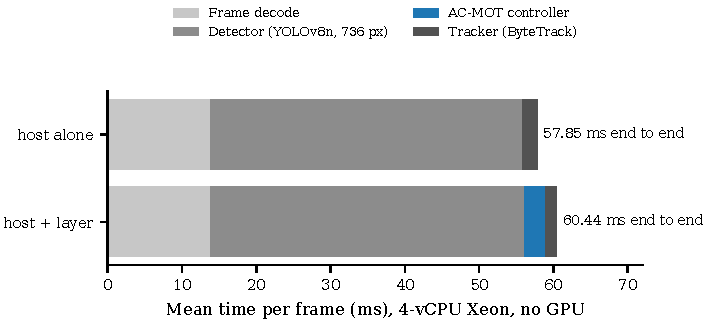
\includegraphics[width=0.66\textwidth]{figures/ch5_fig7_runtime.pdf}
\caption{Mean per-frame time by stage without and with the layer.}
\label{fig:ch5-runtime}
\end{figure}

\section{Failure Cases}\label{sec:ch5-failures}

\subsection{False noisy calls in short streams}
The significant external loss, C-TWiX on KITTI cars ($-1.52$ HOTA), is concentrated in one sequence: in sequence 0014 the layer classified 45 of 106 frames as noisy and HOTA fell by 17.09 points, while six of the other eight sequences changed by less than 0.4 points (Fig.~\ref{fig:ch5-regimes}b). In this short sequence the whole-stream median of $\rho$ had little history to stabilize it, and the noisy regime's band restrictions most likely removed detections that the coordinate-based association relies on; the mechanism was not isolated further. The same sequence accounts for the pedestrian loss (8.50 points). A cold-start protection that requires a minimum amount of history before a noisy call is a natural remedy, but it was not part of the frozen configuration and is left to future work.

\subsection{Under-confident detectors with low-threshold trackers}
With YOLOv8n on KITTI, whose scores are low but mostly correct, the stream is classified noisy ($\rho\approx0.45$), and the noisy regime's rule that only the primary band may start tracks removes true births for ByteTrack and BoT-SORT. MOTA fell by 1.87 and 2.43 while identity switches fell by 271 and 227. A host-relative band that fixed this cell let false tracks through on a noisy aerial stream and was rejected (Table~\ref{tab:ch5-ablation}).

\subsection{Coordinate-only association on DanceTrack}
C-TWiX on DanceTrack lost 1.00 HOTA with an interval including zero, with two sequences losing more than 10 points and one gaining 9.37. The regime was clean on essentially every frame, so the effect comes from the clean-regime operations (cross-class duplicate removal, threshold lowering to $t_2$, and the continuation rescue) acting on a tracker that learns association from coordinates; which of them causes the loss was not isolated.

\section{Limitations}\label{sec:ch5-limits}
\begin{enumerate}
\item The strongest evidence is development evidence. Only PD-SORT, Hybrid-SORT, C-TWiX, and TrackTrack are external, and only PD-SORT improved.
\item No head-to-head comparison with per-frame adaptive-threshold trackers \cite{ma2023adaptivebytetrack,shim2024adaptrack,act2026adaptive} was run. The closest baseline evaluated is the always-intervening prior design, which uses the same score statistics in every frame without a regime decision (Table~\ref{tab:ch5-ablation}).
\item The external systems were evaluated on validation splits with the authors' released detections; no test-server result is reported.
\item The motion rule could not be evaluated on the external systems, whose adapters had no image cue.
\item The aerial evaluation planned for the frozen layer could not be completed because the benchmark data could not be downloaded in the evaluation environment; no aerial claim is therefore made for the frozen layer.
\item Runtime was measured on one general-purpose processor without a graphics processor; no embedded or flight hardware was tested.
\item Reproductions on processors instead of graphics processors differ from the authors' numbers by up to 0.8 HOTA; all comparisons are paired within one environment.
\end{enumerate}

\section{Summary}\label{sec:ch5-conclusions}
This chapter presented a training-free control layer that self-calibrates from a detector's score stream, estimates whether the stream is clean or noisy, and adapts a frozen tracker's input and thresholds through a declared host contract. One frozen configuration was evaluated on nine published trackers, four sources of detections, and three datasets, with development and external evidence kept separate. The layer improved single-stage trackers, including a predeclared external one by 0.61 HOTA points; it restored trackers whose thresholds no longer matched a shifted detector confidence scale; and it raised the multi-object tracking accuracy of two-stage trackers with a noisy detector by 6 to 8 points. On well-matched two-stage pipelines it left the output unchanged, which removed the degradation of the prior design. It failed on a short stream with few candidates, where false noisy calls cost one external tracker 1.52 HOTA points, and on an under-confident detector with low-threshold trackers. For tracking pipelines in which detectors are exchanged more often than trackers are retuned, the layer provides a way to keep published trackers operating without labelled recalibration, together with an explicit record of where it should not be expected to help.


\chapter{Conclusions and Future Work}\label{ch:conclusions}

This thesis studied training-free, causal control of the operating points of multi-object tracking pipelines. It reviewed real-time detection and tracking, established a common evaluation methodology, and presented two controllers: a scene-adaptive controller of the detector operating point for UAV video, and a self-calibrating layer that adapts a frozen tracker to the score stream of a frozen detector. This chapter compares the two approaches, answers the research questions, states the limitations of the thesis as a whole, and outlines future work.

\section{Comparison of the Two Controllers}\label{sec:c-compare}
Table~\ref{tab:c-compare} places the two controllers side by side. They share their principles, namely no learned weights, causal operation, a frozen configuration, and paired statistics, but they differ in what they observe, what they change, and what their evidence shows.

\begin{table}[tbp]
\centering
\caption{The two controllers of the thesis.}
\label{tab:c-compare}
\small\setlength{\tabcolsep}{4pt}
\begin{adjustbox}{max width=\textwidth}
\begin{tabular}{>{\raggedright\arraybackslash}p{3.1cm}>{\raggedright\arraybackslash}p{5.6cm}>{\raggedright\arraybackslash}p{5.6cm}}
\toprule
 & Scene-adaptive controller (Chapter~\ref{ch:scene}) & Self-calibrating layer (Chapter~\ref{ch:layer}) \\
\midrule
Observes & five image and detection cues, ranked against a calibration set & the stream of detector scores of the previous ten frames \\
Changes & detector confidence, suppression, and resolution & candidates passed to the tracker, their scores, the tracker's thresholds and matching tolerance \\
Calibration & label-free calibration set from one detector; parameters selected on validation data & none beyond the tracker's declared host contract \\
Pipelines & one detector (YOLOv8n) and one tracker (ByteTrack) & nine published trackers, four sources of detections \\
Data & VisDrone2019, UAVDT & MOT17, KITTI, DanceTrack \\
Main gain & $+5.41$ HOTA over the static default on held-out data & recovery from confidence shift; $+0.61$ HOTA on single-stage trackers \\
Main finding & gain equals that of the matched static operating point & self-limiting: no change on well-matched two-stage pipelines \\
Main failure & more identity switches than the hand-designed controller & false noisy decisions in a short sequence ($-1.52$ HOTA) \\
Cost & 38.98 FPS end to end on a T4, decoding excluded & 2.95 ms per frame on a four-core processor \\
\bottomrule
\end{tabular}
\end{adjustbox}
\end{table}

The two studies are complementary. The first showed that the largest accessible gain in a fixed pipeline is to calibrate its operating point on representative data, and that switching adds little once the operating point is right. The second showed that the operating point can be kept right without labels when the detector changes, provided that the controller reads the detector's scores rather than the image, acts on the tracker rather than on the detector, and restrains itself when the pipeline already fits.

\section{Answers to the Research Questions}\label{sec:c-answers}

\paragraph{RQ1.} A training-free scene-adaptive controller, selected on seven validation sequences and frozen before testing, improved held-out HOTA on VisDrone2019 test-dev from 28.43 to 33.84 percent over a static default and from 32.70 to 33.84 percent over a hand-designed controller, and it transferred to UAVDT without retuning (24.08 to 28.39 percent). The improvement did not come from adaptation. A matched static operating point reached 33.93 percent on test-dev, and the difference of $-0.09$ points had an interval that includes zero. The validation search had converged to a near-static controller at the top of the accuracy--resolution curve, where switching cannot help. Scene-driven switching did add accuracy for the hand-designed controller, whose resolution range lies on the steep part of that curve, which indicates that switching pays off when the throughput budget does not admit the best static operating point.

\paragraph{RQ2.} A training-free layer that self-calibrates from the detector's score stream kept published trackers operating under detector confidence shift: when the detector scores were halved, it restored two trackers from 0 to 66.17 and 66.72 HOTA. With a noisy detector on KITTI it raised the MOTA of two two-stage trackers by 5.98 and 7.86 points. It raised the HOTA of the single-stage OC-SORT and of the predeclared external PD-SORT by 0.61 points, with intervals above zero, by supplying the continuation stage that these trackers lack. On five trackers with a low-score stage and well-matched detections it changed HOTA by at most 0.06 points or not at all, which is the intended self-limiting behavior. On the post-freeze external systems the evidence is mixed and small: C-TWiX lost 1.52 HOTA on KITTI cars, concentrated in one short sequence with false noisy decisions, and TrackTrack changed by a significant but negligible $-0.013$ points. The layer therefore does what it was designed to do on the failure modes it targets, and it does not improve every tracker.

\section{Limitations}\label{sec:c-limits}
The limitations of each study are stated in Sections~\ref{sec:ch4-limits} and~\ref{sec:ch5-limits}. Four limitations apply to the thesis as a whole.
\begin{enumerate}
\item \emph{No common benchmark for the two controllers.} The scene-adaptive controller was evaluated on aerial data, and the self-calibrating layer on ground-level data. The aerial evaluation planned for the frozen layer could not be completed because the benchmark data could not be downloaded in the evaluation environment, so the thesis makes no aerial claim for the layer and no direct comparison of the two controllers on the same data.
\item \emph{Hardware.} Throughput was measured on a Tesla T4 and on a general-purpose processor. No embedded flight computer was tested, and no flight test was performed.
\item \emph{Detector fine-tuning.} All detectors were COCO-pretrained or released by the tracker authors; no detector was fine-tuned on aerial data, which bounds the absolute accuracy of Chapter~\ref{ch:scene}.
\item \emph{Statistical resolution.} With 7 to 25 sequences per evaluation cell, differences of a few tenths of a HOTA point are generally not resolved, and most of the layer's gains come from development cells rather than from external systems.
\end{enumerate}

\section{Future Work}\label{sec:c-future}
The results suggest the following directions.
\begin{enumerate}
\item \emph{Cold-start protection.} The largest external failure of the layer came from noisy decisions made with little history in a short sequence. Requiring a minimum amount of history before a noisy decision is a natural remedy; it must be declared and evaluated on new external data, not tuned on the failure case.
\item \emph{Aerial evaluation of the layer.} Evaluating the frozen layer on VisDrone and UAVDT, with the same detectors and trackers as Chapter~\ref{ch:scene}, would test it where scene and confidence changes occur together, and would allow a direct comparison with the scene-adaptive controller.
\item \emph{Combining the two controllers.} The two controllers act on different parts of the pipeline and could run together: a calibrated detector operating point for throughput and recall, and the score-driven layer for robustness to detector changes. Whether their effects add up is an open question.
\item \emph{Constrained hardware.} Chapter~\ref{ch:scene} indicates that scene-driven switching is most useful when the throughput budget does not admit the best static operating point. Embedded processors are that regime, and they are the natural setting in which to revisit adaptive resolution.
\item \emph{Broader detector shifts.} The confidence-shift experiments used monotone transforms of fixed detections and two live detectors. Quantized, pruned, and domain-shifted detectors would test the layer's premise more directly.
\item \emph{Other tracker families.} End-to-end trackers that predict identities directly \cite{zeng2022motr,gao2025motip} expose different thresholds; extending the host contract to them would test how far the layer's design generalizes.
\end{enumerate}

\section{Concluding Remarks}\label{sec:c-final}
Tracking pipelines are built from components that were tuned separately, and their operating points are the place where those components meet. This thesis found that calibrating that meeting point matters more than adapting it frame by frame, and that it can be kept calibrated without labels when a component changes. Both findings were obtained with configurations frozen before testing and with the failures reported alongside the gains, which is the standard the thesis set for itself.


\bibliographystyle{unsrtnat}
\bibliography{references}

\appendix
\chapter{Reproducibility Details}\label{app:repro}

This appendix lists the software, frozen artifacts, and settings needed to reproduce the results of Chapters~\ref{ch:scene} and~\ref{ch:layer}. All code, configurations, protocol files, and result records are kept in the project's version-control repository.

\section{Common Settings}
\begin{longtable}{@{}p{4.6cm}p{9.8cm}@{}}
\toprule
Item & Setting \\
\midrule
Evaluation library & TrackEval, commit 12c8791 \\
Bootstrap & percentile bootstrap over sequences, seed 42; 5,000 resamples (Chapter~\ref{ch:scene}), 10,000 resamples (Chapter~\ref{ch:layer}) \\
Significance & 95\% interval excludes zero \\
Tie (Chapter~\ref{ch:layer}) & $|\Delta\mathrm{HOTA}|<0.01$ \\
\bottomrule
\end{longtable}

\section{Scene-Adaptive Controller (Chapter~\ref{ch:scene})}
\begin{longtable}{@{}p{4.6cm}p{9.8cm}@{}}
\toprule
Item & Setting \\
\midrule
Detector & Ultralytics YOLOv8n, COCO-pretrained, library version 8.3.200, half precision, at most 1000 detections per frame \\
Classes & person, car, bus, truck (VisDrone); car, bus, truck (UAVDT) \\
Tracker & Ultralytics ByteTrack with score fusion, nominal frame rate 30 \\
Tracker profiles & default: high 0.25, low 0.10, new 0.25, buffer 30, match 0.80; tuned: high 0.18, low 0.04, new 0.20, buffer 45, match 0.86 \\
Processor & one NVIDIA Tesla T4 \\
Calibration set & 288 samples, every tenth frame of the 7 VisDrone validation sequences; anchor operating point 960 pixels, confidence 0.35, suppression 0.35 \\
Temporal settings & analysis stride $K=10$ frames, smoothing window $W=7$ analyses \\
Resolution levels & 512, 928, 960 pixels \\
Quality profile Q & trial 24 of the single-objective search; confidence 0.30 to 0.40, suppression 0.35, resolution thresholds 0.135 and 0.287 \\
Balanced profile B & trial 22 of the multi-objective search; confidence 0.40, suppression 0.60 to 0.35, resolution thresholds 0.293 and 0.666 \\
Search & tree-structured Parzen estimator (Optuna), at most 50 trials, throughput gate 25 FPS \\
Ground-truth filter (VisDrone) & categories pedestrian, car, van, truck, bus; considered; occlusion and truncation below 2; class-agnostic \\
Frozen code & version-control tag \texttt{v1.0.0-acmot-frozen} \\
\bottomrule
\end{longtable}

\section{Self-Calibrating Layer (Chapter~\ref{ch:layer})}
\begin{longtable}{@{}p{4.6cm}p{9.8cm}@{}}
\toprule
Item & Setting \\
\midrule
Frozen configuration & V7f; version-control tag \texttt{universal-acmot-v7-freeze} (commit 488df9a) \\
Lock & file of cryptographic hashes of the layer, its configuration, and the evaluation runners, verified before every post-freeze run \\
Automated tests & 61 tests (causality, state reset, pass-through, name independence, affine invariance, lock integrity) \\
Score statistics & logits of all candidates of the previous $W=10$ frames; nested exact Otsu thresholds \\
Regime & clean if the median of $\rho$ over all past non-cold frames is at least 0.5 \\
Noisy score remap & stream ECDF; primary band to $[0.5,1)$, extension band to $[0.1,0.5)$; association and birth thresholds 0.5 \\
Duplicate overlap & IoU 0.5 \\
Rescue overlap & IoU 0.5 with a track of the previous frame \\
Motion rule & phase correlation on a quarter-resolution frame; $m_t=\min(0.95,1-(1-m_0)/\max(1,r_t))$; history of 100 motion ratios \\
Runtime processor & 4-vCPU Intel Xeon, 2.10 GHz, no graphics processor \\
Reproduction classes & EXACT $|\Delta\mathrm{HOTA}|\le 0.2$; CLOSE $\le 1.0$ with a documented, untuned cause; FAILED otherwise \\
\bottomrule
\end{longtable}


% Arabic summary and Arabic title page (source: arabic/arabic_summary.tex, built with LuaLaTeX)
\cleardoublepage
\phantomsection
\addcontentsline{toc}{chapter}{Arabic Summary}

\includepdf[pages=-,pagecommand={\thispagestyle{empty}}]{arabic/arabic_summary.pdf}

\end{document}
